%%
%% This is file `mcmthesis-demo.tex',
%% generated with the docstrip utility.
%%
%% The original source files were:
%%
%% mcmthesis.dtx  (with options: `demo')
%%
%% -----------------------------------
%%
%% This is a generated file.
%%
%% Copyright (C)
%%       2010 -- 2015 by Zhaoli Wang
%%       2014 -- 2019 by Liam Huang
%%       2019 -- present by latexstudio.net
%%
%% This work may be distributed and/or modified under the
%% conditions of the LaTeX Project Public License, either version 1.3
%% of this license or (at your option) any later version.
%% The latest version of this license is in
%%   http://www.latex-project.org/lppl.txt
%% and version 1.3 or later is part of all distributions of LaTeX
%% version 2005/12/01 or later.
%%
%% This work has the LPPL maintenance status `maintained'.
%%
%% The Current Maintainer of this work is Liam Huang.
%%
%%
%% This is file `mcmthesis-demo.tex',
%% generated with the docstrip utility.
%%
%% The original source files were:
%%
%% mcmthesis.dtx  (with options: `demo')
%%
%% -----------------------------------
%%
%% This is a generated file.
%%
%% Copyright (C)
%%       2010 -- 2015 by Zhaoli Wang
%%       2014 -- 2019 by Liam Huang
%%       2019 -- present by latexstudio.net
%%
%% This work may be distributed and/or modified under the
%% conditions of the LaTeX Project Public License, either version 1.3
%% of this license or (at your option) any later version.
%% The latest version of this license is in
%%   http://www.latex-project.org/lppl.txt
%% and version 1.3 or later is part of all distributions of LaTeX
%% version 2005/12/01 or later.
%%
%% This work has the LPPL maintenance status `maintained'.
%%
%% The Current Maintainer of this work is Liam Huang.
%%
\documentclass{mcmthesis}
\mcmsetup{CTeX = false,    % 使用 CTeX 套装时，设置为 true
          tcn = {2517063}, problem = \textcolor{red}{C},
          sheet = true, titleinsheet = true, keywordsinsheet = true,
          titlepage = false, abstract = false}
        
\usepackage{newtxtext}     % \usepackage{palatino}
\usepackage[backend=bibtex]{biblatex}   % for RStudio Complie
\usepackage{booktabs}
\usepackage{colortbl}
\usepackage{underscore}
\usepackage{tocloft}
\usepackage{float}
\usepackage{enumitem}
\usepackage{multirow}
\usepackage{epstopdf}
\usepackage{subcaption}
\usepackage{caption}
\usepackage{vcell}
\setlength{\cftbeforesecskip}{6pt}
\renewcommand{\contentsname}{\hspace*{\fill}\Large\bfseries Contents \hspace*{\fill}}

\title{Enjoy a Cozy and Green Bath}
% \author{\small \href{http://www.latexstudio.net/}
%   {\includegraphics[width=7cm]{mcmthesis-logo}}}
\date{\today}

\begin{document}

\begin{abstract}

XXXX

XXXX, \textbf{XXX}

XXXX

\begin{keywords}
Heat transfer; Thermodynamic system; CFD; Energy conservation
\end{keywords}

\end{abstract}

\maketitle

%% Generate the Table of Contents, if it's needed.
% \renewcommand{\contentsname}{\centering Contents}
\tableofcontents   % 若不想要目录, 注释掉该句
\thispagestyle{empty}

\newpage

\section{Introduction}

\subsection{Problem Background}

The Olympic Games is one of the most influential sporting events globally. It not only showcases the outstanding talents of athletes but also promotes cultural exchanges and cooperation among nations. Since the revival of the modern Olympics in 1896, the Games has become an important platform for countries to display their athletic prowess. The medal table has always been an integral part of the Olympics, reflecting not only the sports levels of different countries but also being closely related to their economic, social, and cultural development. The number and rank of medals are often seen as one of the symbols of a country's comprehensive national strength. The medal table of the 2024 Paris Olympics shows the competitive landscape of countries in terms of gold medals and total medals. For example, the United States ranked first in total medals, while China and the United States were tied for first in gold medals. The host country, France, also performed well, ranking fourth. In addition, some countries such as Albania, Cabo Verde, Dominica, and Saint Lucia won medals for the first time in the Olympics, which reflected the diversity and inclusiveness of the Games.

\begin{figure}[h] 
\centering
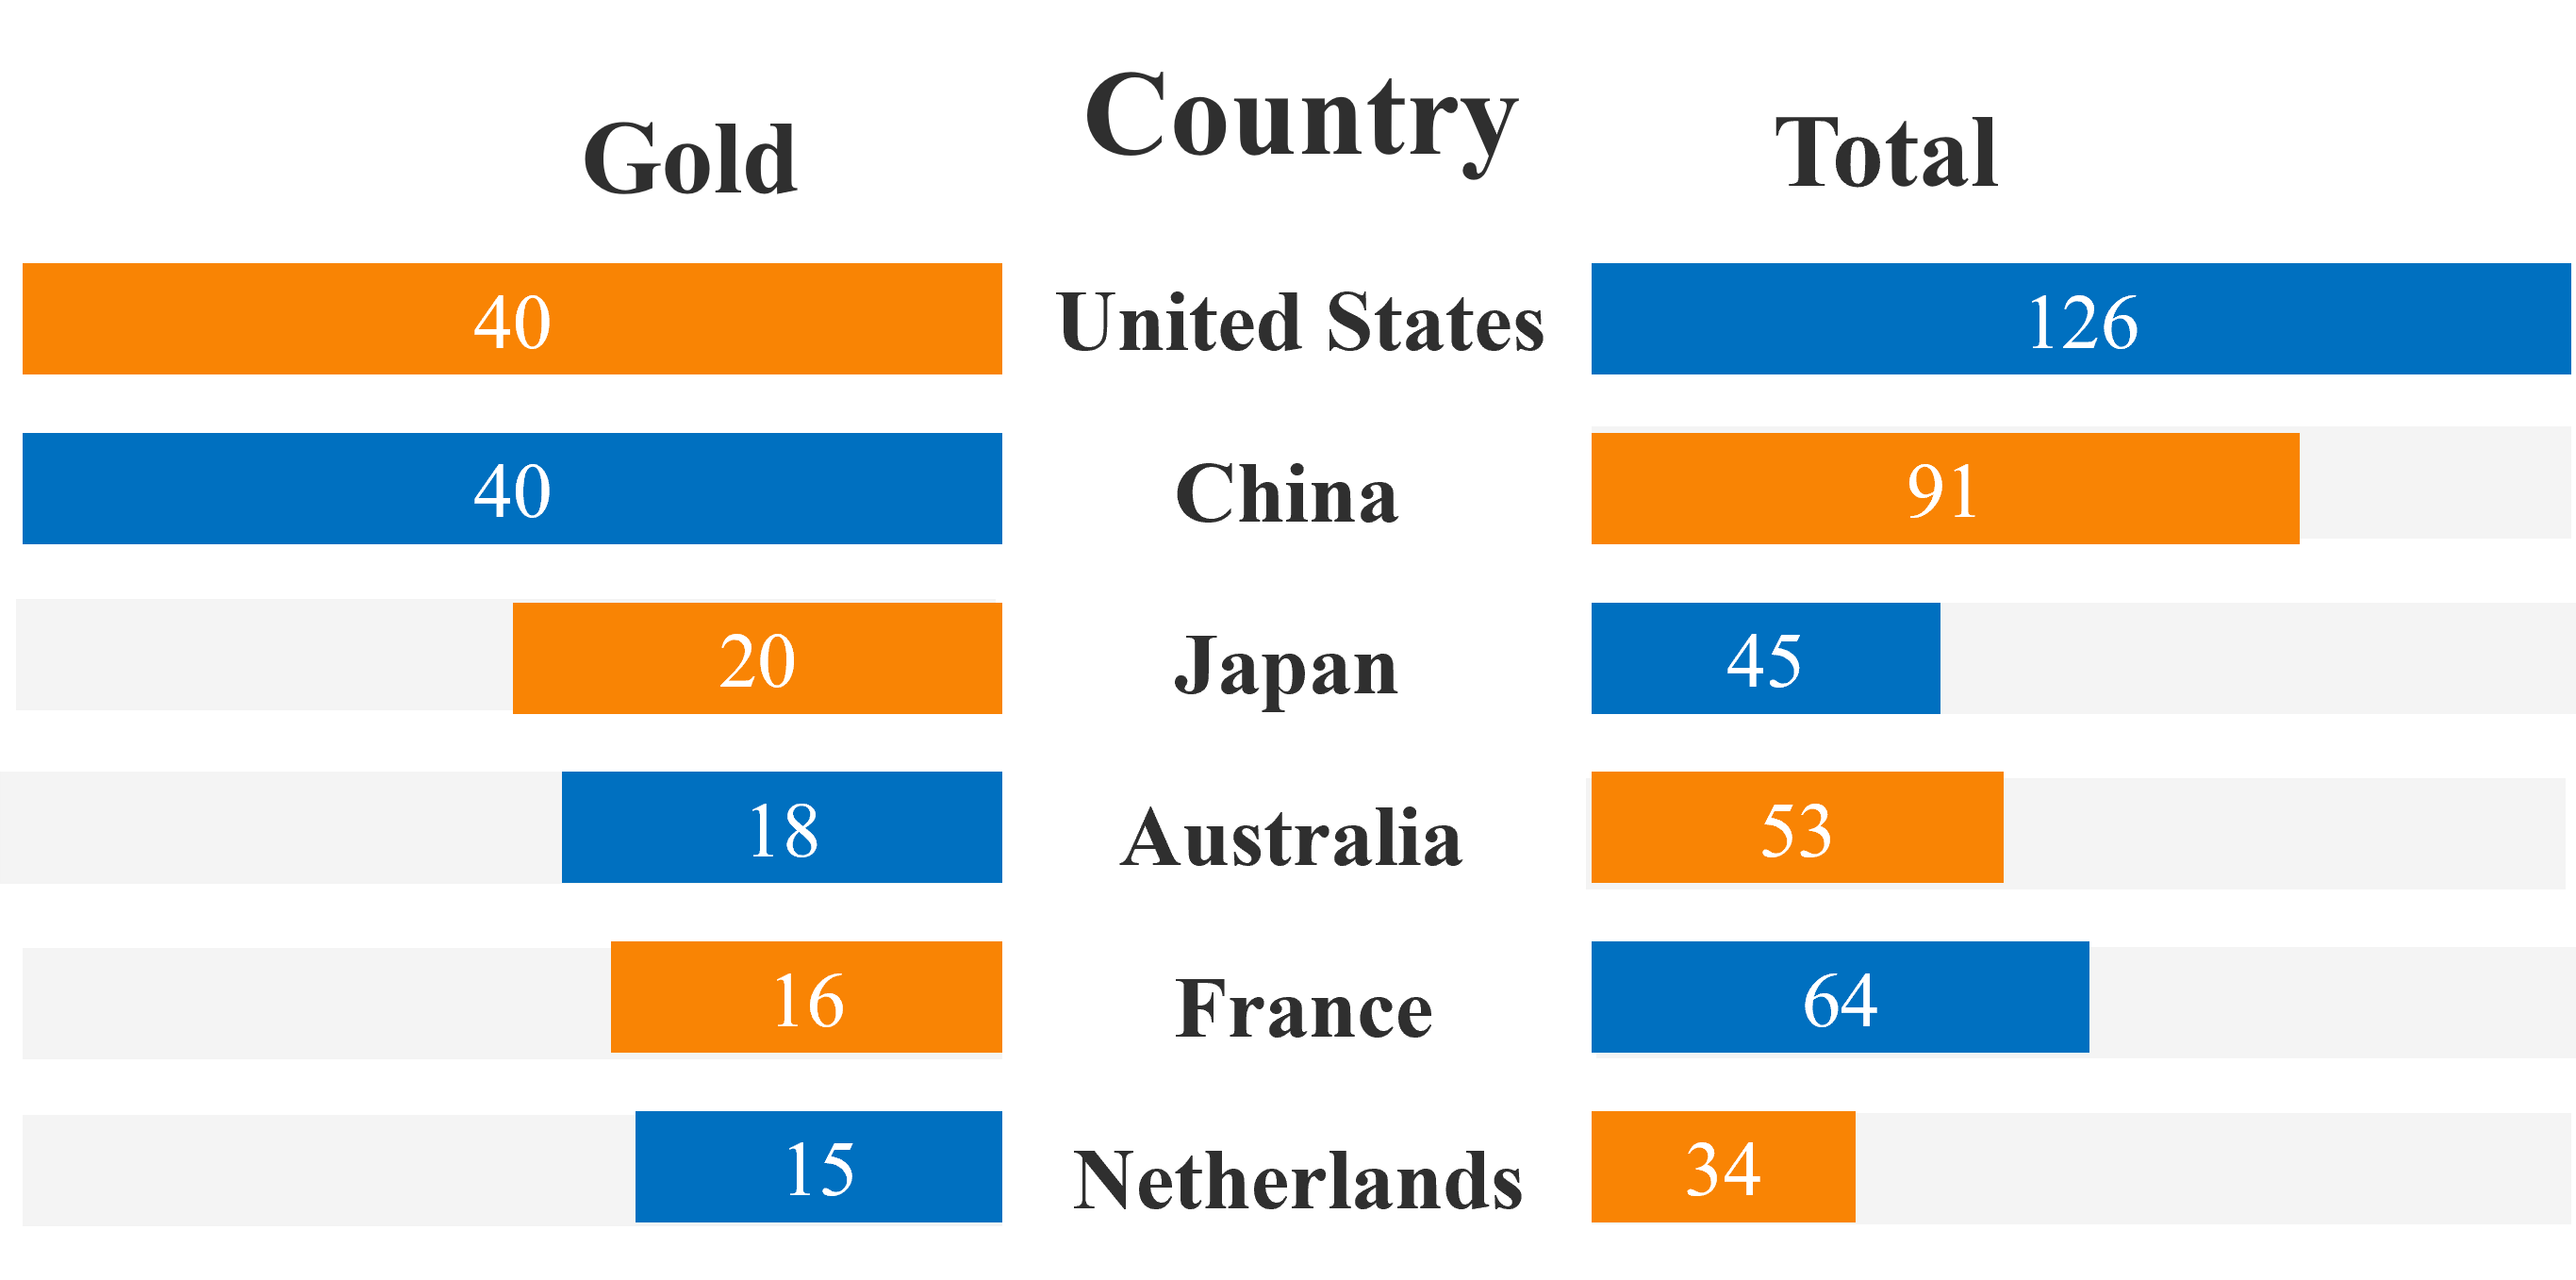
\includegraphics[width=0.8\linewidth]{Paris Olympics(2024) Medal Table - Gold Medals Top 6 Countries.png}
\caption{Paris Olympics(2024) Medal Table - Gold Medals Top 6 Countries}
\end{figure}

\begin{figure}[htbp]
	\centering
	\begin{minipage}{0.4\linewidth}
		\centering
		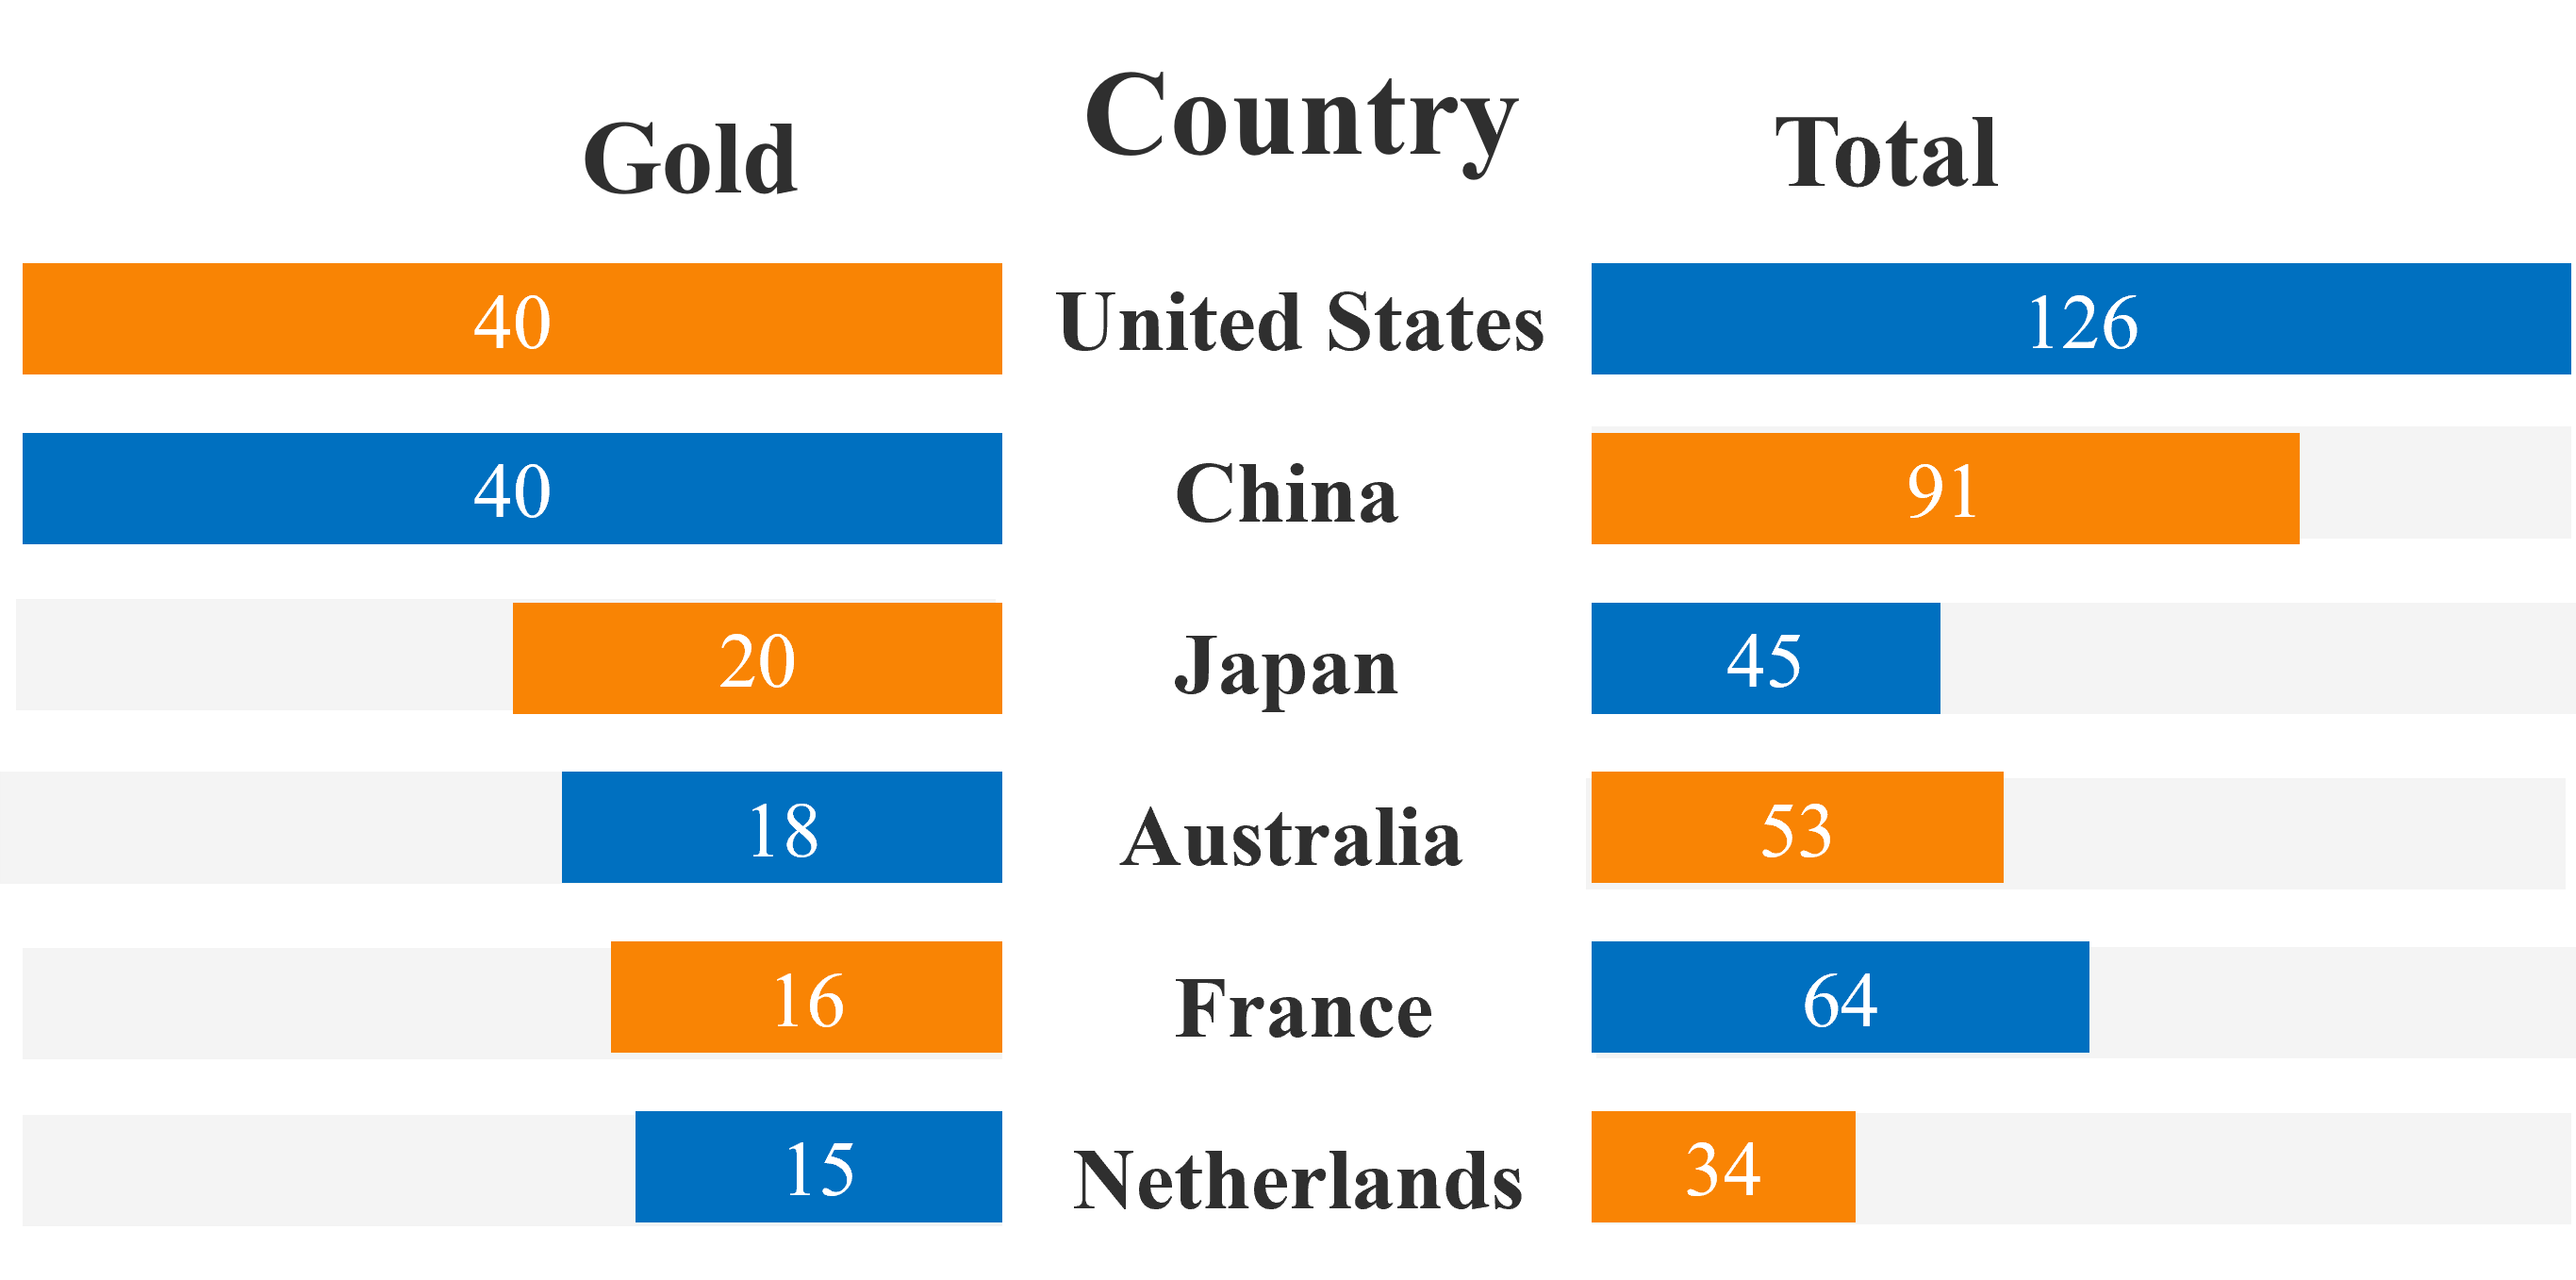
\includegraphics[width=1\linewidth]{Paris Olympics(2024) Medal Table - Gold Medals Top 6 Countries.png}
		\caption{Paris Olympics(2024) Medal Table - Gold Medals Top 6 Countries}
	\end{minipage}
	\begin{minipage}{0.4\linewidth}
		\centering
		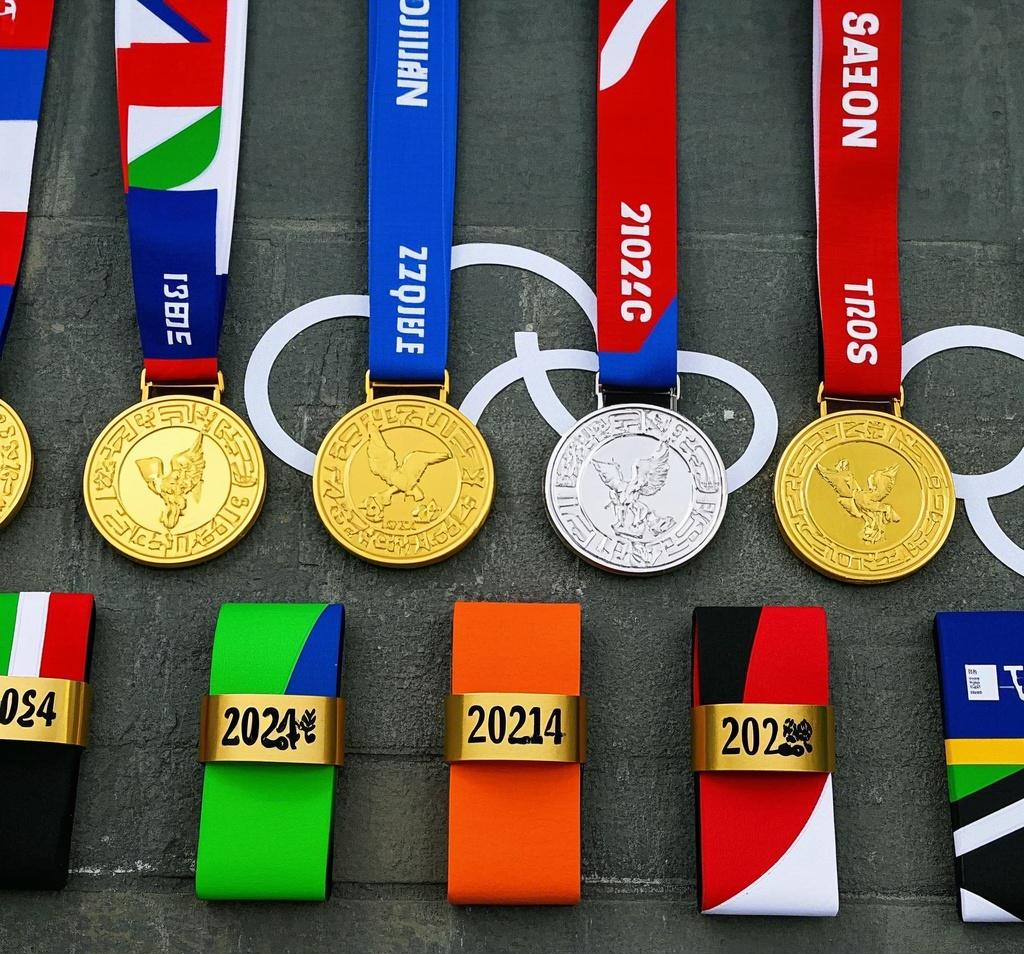
\includegraphics[width=1\linewidth]{R-C.png}
		\caption{XXX?}
	\end{minipage}
\end{figure}

\subsection{Restatement of the Problem}

{\bf Question 1: Development of the Medal Quantity Prediction Model} 

$\star$ Develop a model to predict the number of medals (at least including gold medals and total medals) that each country will win at the 2028 Los Angeles Olympics. In addition, assess the uncertainty and prediction accuracy of the model, and provide prediction intervals.

$\star$ Predict which countries may improve in 2028 and which may perform worse than in 2024.

$\star$ Consider countries that have not yet won medals, and predict how many countries may win medals for the first time in 2028, along with probability estimates.

$\star$ The model should also explore the relationship between the setting of Olympic events and the medal-winning situations of various countries, and discuss the impact of the host country's event selection on the medal table. Identify which sports contribute the most to the medal counts of different countries and explain the reasons.

{\bf Question 2: "Great Coach" Effect Analysis}

$\star$ Identify the impact of "great coach" on the number of medals through data analysis.

$\star$ Estimate the proportion of this effect on the number of medals.

$\star$ Select three countries and analyze which sports they require the introduction of  "great coach", and estimate the potential impact.

{\bf Question 3:Other Original Insights}

$\star$ Provide other original insights revealed by the model regarding the Olympic medal table.

$\star$ Explain how these insights can provide decision support for country Olympic Committees.

\subsection{Our Work}
We put forward three models to mine the information of the reported result data. The structure of our paper is shown in Figure XXX.

\begin{figure}[h] 
\centering
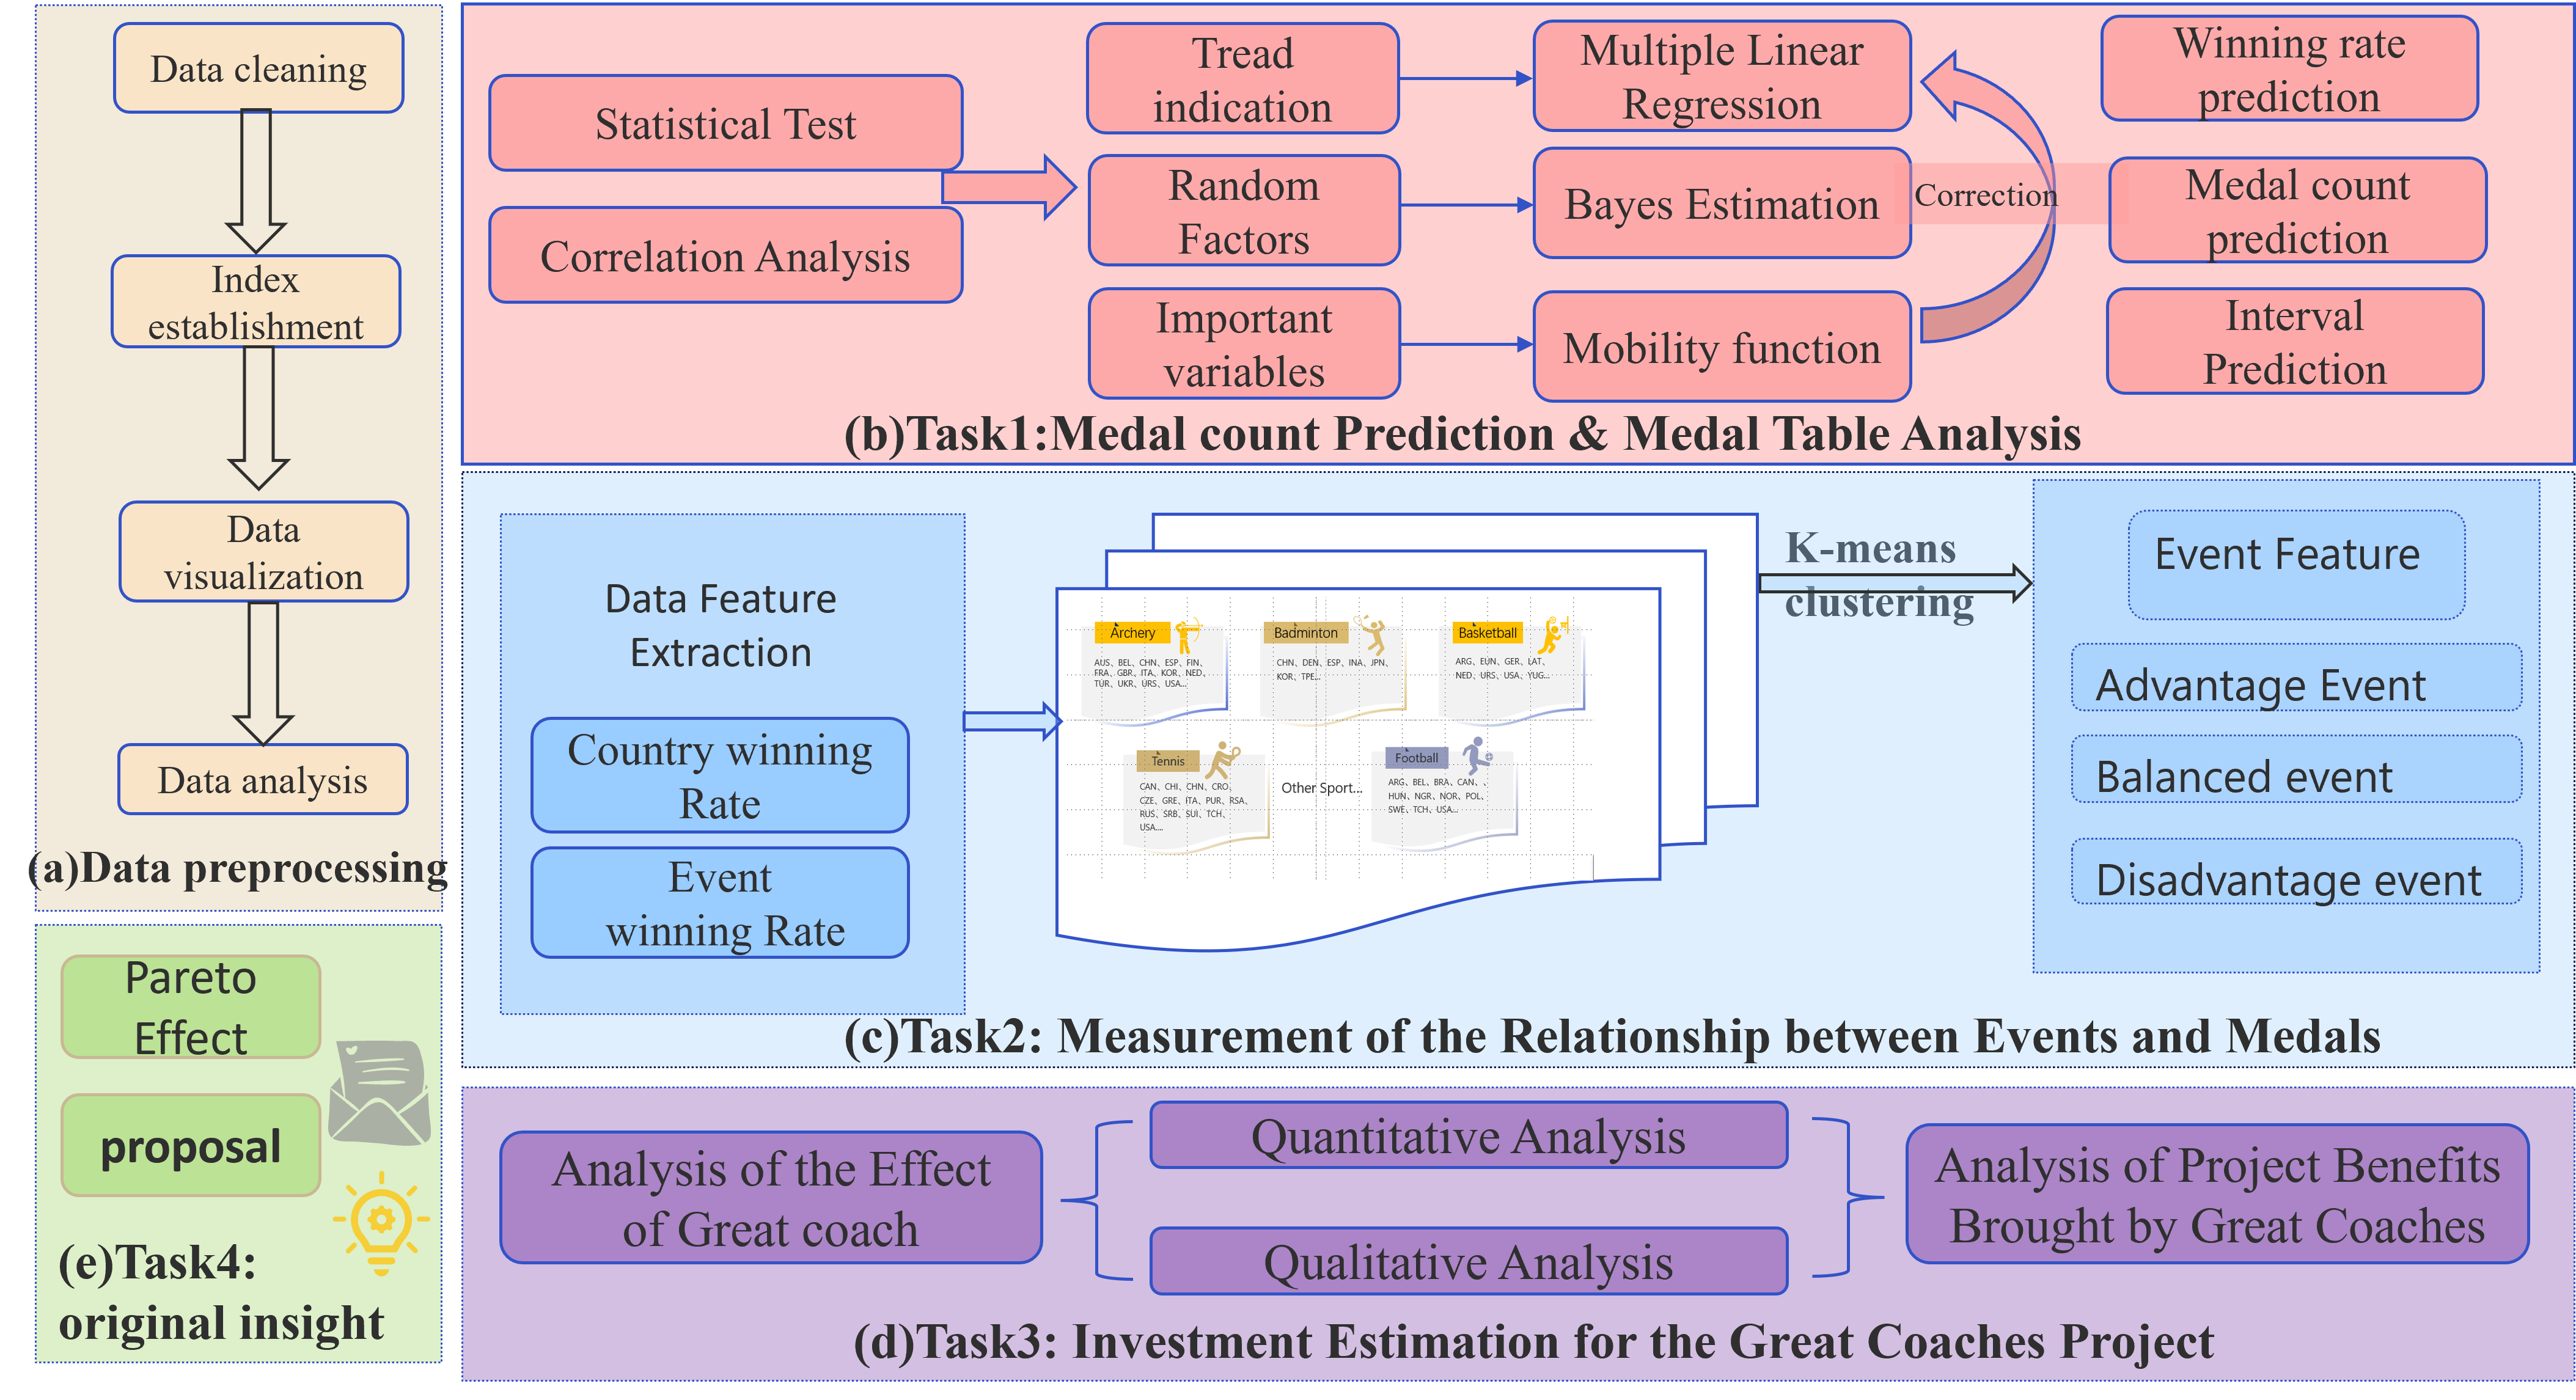
\includegraphics[width=0.8\linewidth]{Our Work.png}
\caption{Our Work}
\end{figure}

\section{Assumptions and Justification}

To simplify the problem and make it convenient for us to simulate real-life conditions, we make the following basic assumptions, each of which is properly justified.

$  \blacklozenge $  {\bf Assumption 1: XXXXX.}

{\bf Justification:} XXXXX

$  \blacklozenge $  {\bf Assumption 2: XXXXX.}

{\bf Justification:} XXXXX

$  \blacklozenge $  {\bf Assumption 3: XXXXX.}

{\bf Justification:} XXXXX

$  \blacklozenge $  {\bf Assumption 4: XXXXX.} 

{\bf Justification:} XXXXX

\section{Notations}

\begin{table}[h]
\centering
\begin{tabular}{ll} 
\hline
\textbf{Symbols~ ~ ~ ~ ~ ~~} & \textbf{Description}                                                                                                                                                                                                                                                                                                                  \\ 
\hline
\vcell{$MP^{i}(t)$}                  & \vcell{\begin{tabular}[b]{@{}l@{}}\textcolor[rgb]{0.031,0.031,0.031}{The proportion of the total number of medals won by }\\\textcolor[rgb]{0.031,0.031,0.031}{the i-th country at the t-th Olympic Games.}\\\textcolor[rgb]{0.031,0.031,0.031}{}\end{tabular}}                                                                       \\[-\rowheight]
\printcelltop                & \printcellmiddle                                                                                                                                                                                                                                                                                                                      \\
\vcell{$S\_Num^{i}(t)$}                  & \vcell{\begin{tabular}[b]{@{}l@{}}\textcolor[rgb]{0.031,0.031,0.031}{The total number of events participated by the i-th~}\\\textcolor[rgb]{0.031,0.031,0.031}{country in the t-th Olympic Games.}\\\textcolor[rgb]{0.031,0.031,0.031}{}\end{tabular}}                                                                                \\[-\rowheight]
\printcelltop                & \printcellmiddle                                                                                                                                                                                                                                                                                                                      \\
\vcell{$P\_Num^{i}(t)$}                  & \vcell{\begin{tabular}[b]{@{}l@{}}\textcolor[rgb]{0.031,0.031,0.031}{The number of awards won by athletes from the i-th }\\\textcolor[rgb]{0.031,0.031,0.031}{country in the t-th Olympic Games.}\\\textcolor[rgb]{0.031,0.031,0.031}{}\end{tabular}}                                                                                 \\[-\rowheight]
\printcelltop                & \printcellmiddle                                                                                                                                                                                                                                                                                                                      \\
\vcell{$M_{i, j}(t)$}                  & \vcell{\begin{tabular}[b]{@{}l@{}}\textcolor[rgb]{0.031,0.031,0.031}{The number of awards won by country i in event j at }\\\textcolor[rgb]{0.031,0.031,0.031}{the t-th Olympic Games.}\\\textcolor[rgb]{0.031,0.031,0.031}{}\end{tabular}}                                                                                           \\[-\rowheight]
\printcelltop                & \printcellmiddle                                                                                                                                                                                                                                                                                                                      \\
\vcell{$S_{i, j}(t)$}                   & \vcell{\begin{tabular}[b]{@{}l@{}}\textcolor[rgb]{0.031,0.031,0.031}{The total number of athletes from country i }\\\textcolor[rgb]{0.031,0.031,0.031}{participating in event j at the t-th Olympic Games.}\\\textcolor[rgb]{0.031,0.031,0.031}{}\end{tabular}}                                                                       \\[-\rowheight]
\printcelltop                & \printcellmiddle                                                                                                                                                                                                                                                                                                                      \\
\vcell{$\hat{MP_{j}^{i}}$}                   & \vcell{\begin{tabular}[b]{@{}l@{}}\textcolor[rgb]{0.031,0.031,0.031}{The j-th predicted value for country i obtained through }\\\textcolor[rgb]{0.031,0.031,0.031}{a multiple linear regression model based on the }\\\textcolor[rgb]{0.031,0.031,0.031}{independent variables.}\\\textcolor[rgb]{0.031,0.031,0.031}{}\end{tabular}}  \\[-\rowheight]
\printcelltop                & \printcellmiddle                                                                                                                                                                                                                                                                                                                      \\
\vcell{$X^{i}(t)$, $Y^{i}(t)$, $Z^{i}(t)$}                  & \vcell{\begin{tabular}[b]{@{}l@{}}\textcolor[rgb]{0.031,0.031,0.031}{The number of gold, silver, and bronze medals won by }\\\textcolor[rgb]{0.031,0.031,0.031}{country i in year t.}\\\textcolor[rgb]{0.031,0.031,0.031}{}\end{tabular}}                                                                                             \\[-\rowheight]
\printcelltop                & \printcellmiddle                                                                                                                                                                                                                                                                                                                      \\
\vcell{$Item_{i, j}(t)$}                   & \vcell{\textcolor[rgb]{0.031,0.031,0.031}{The index of advantage for country i in event j in year t.}}                                                                                                                                                                                                                                \\[-\rowheight]
\printcelltop                & \printcellmiddle                                                                                                                                                                                                                                                                                                                      \\
\hline
\end{tabular}
\end{table}

where we define the main parameters while specific value of those parameters will be given later.

\section{Data Pre-processing}
\subsection{Data Overview}
Conduct a general analysis of the data as shown in Figure 1.

\begin{figure}[h] 
\centering
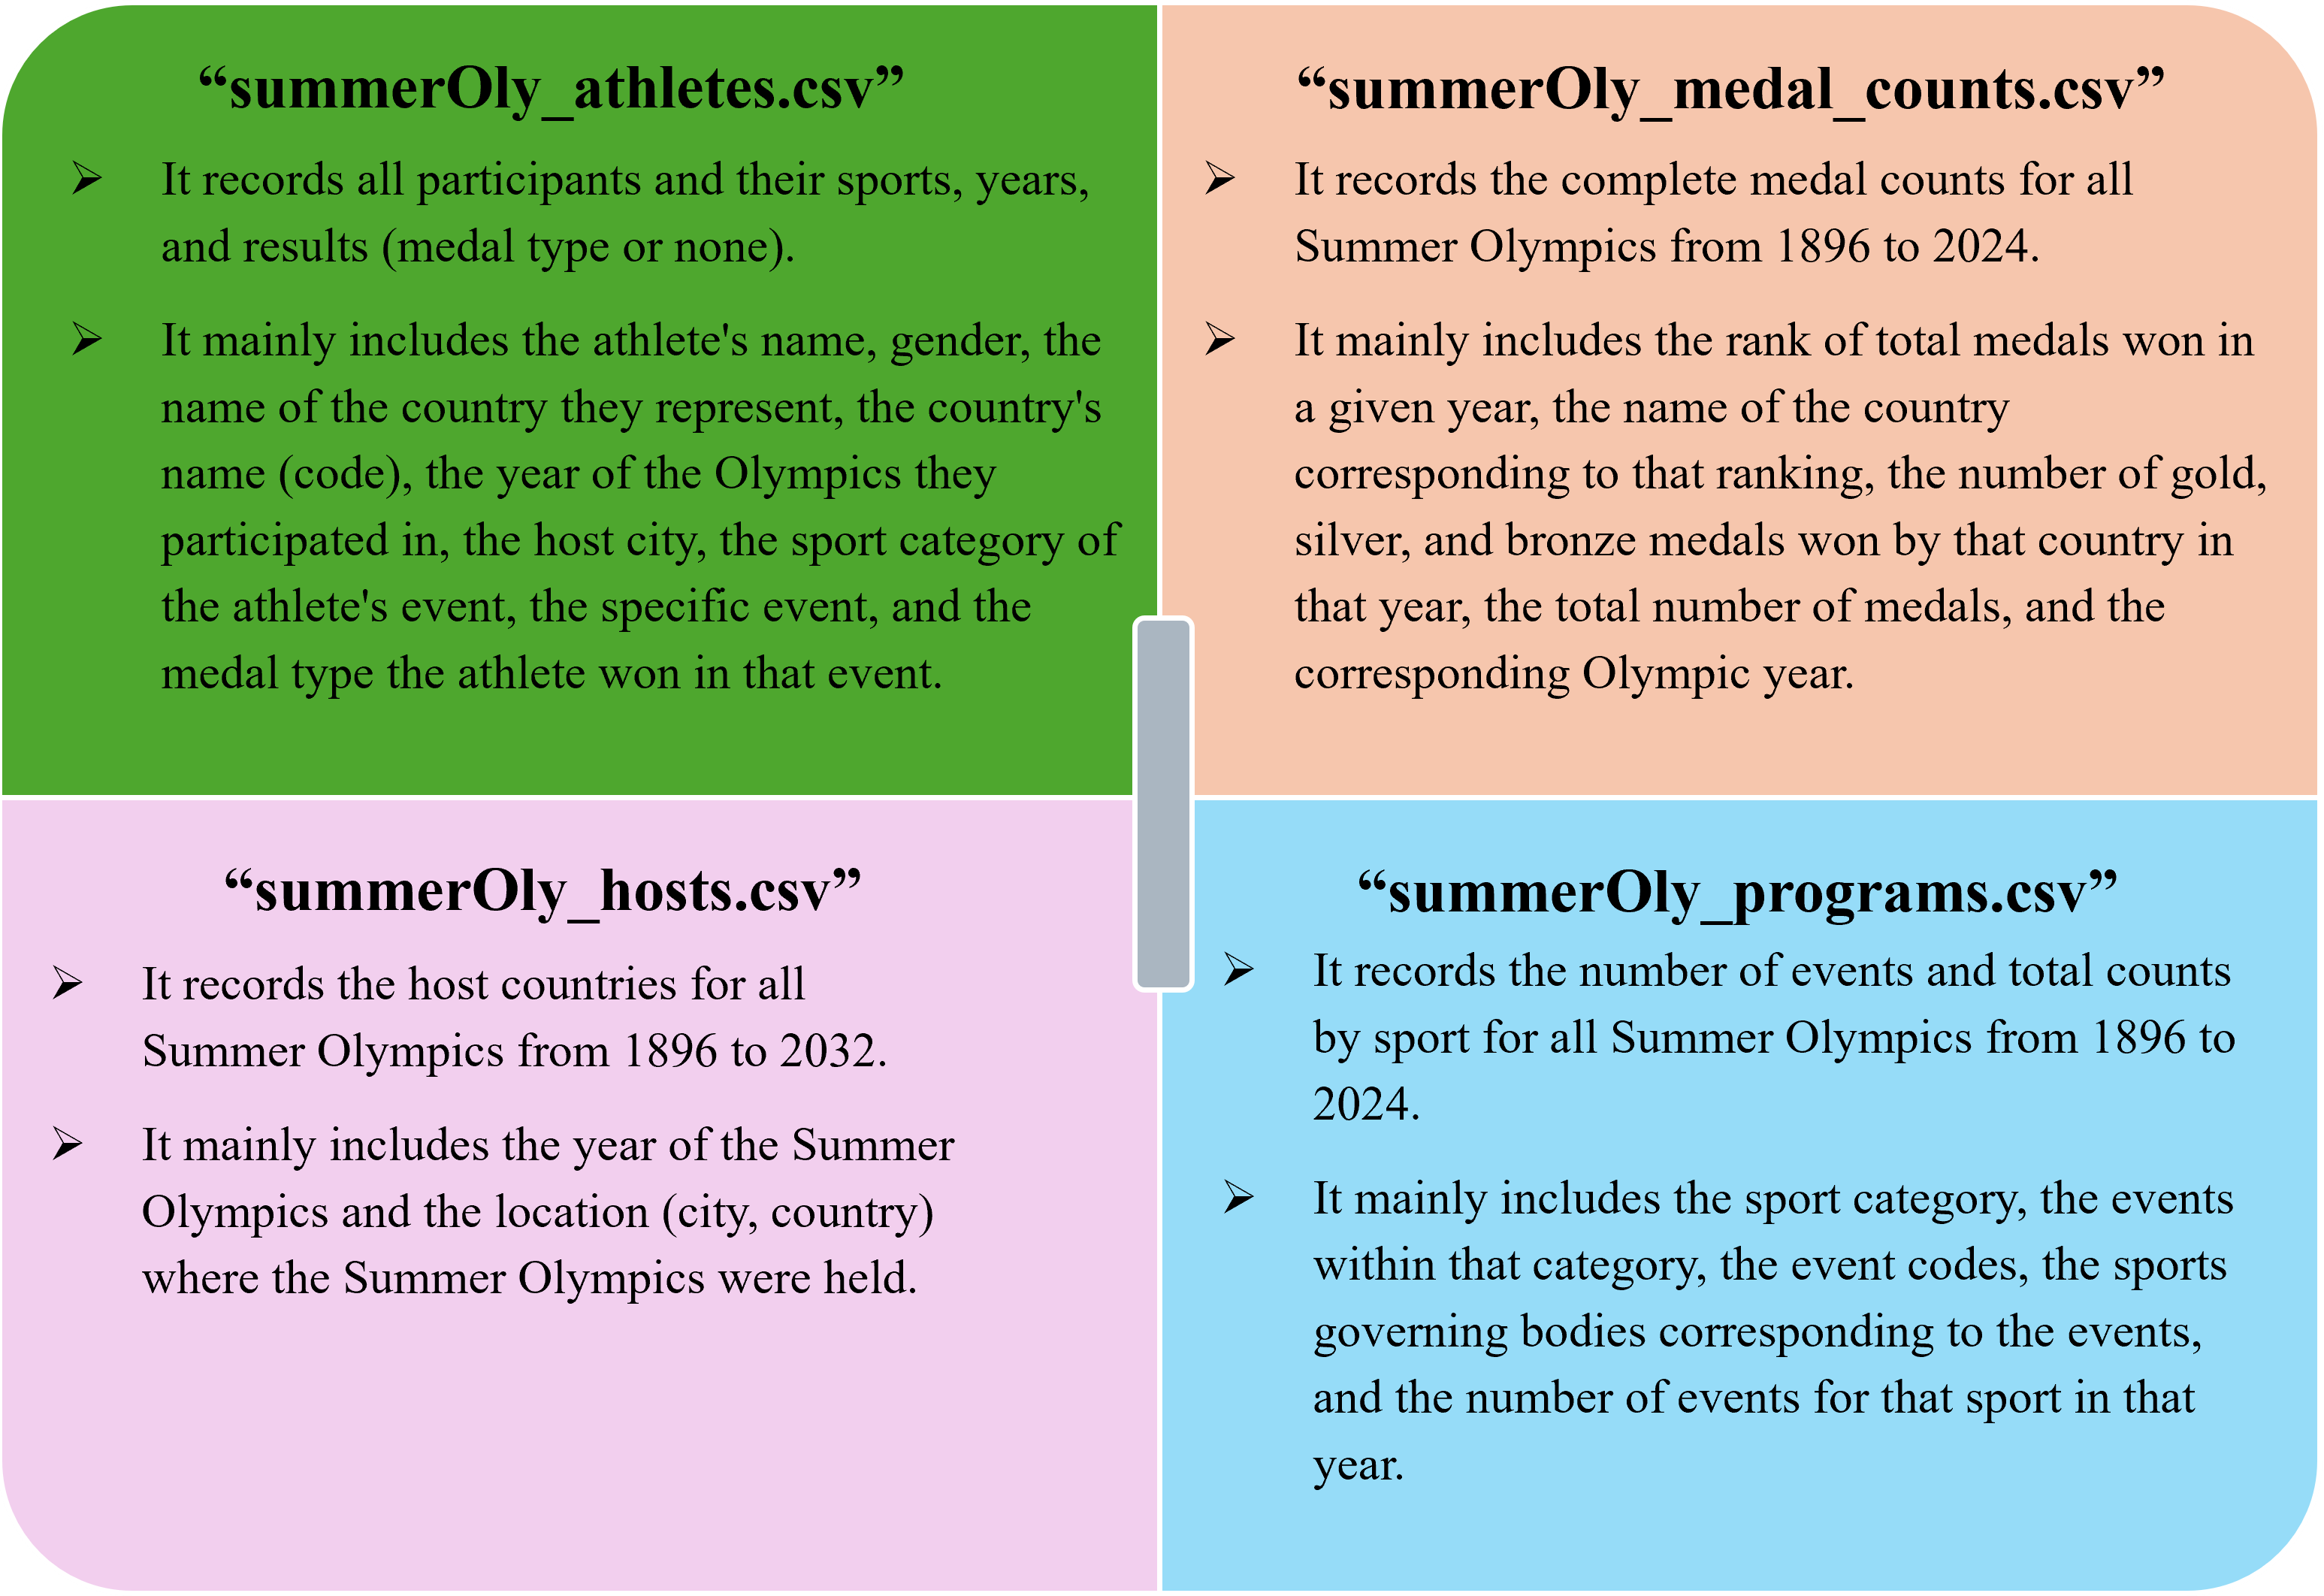
\includegraphics[width=10cm]{Overview of four data tables.png}
\caption{Overview of four data tables} \label{fig1}
\end{figure}

Notably: 

a) In 1936, during Nazi Germany, the Berlin Olympics was boycotted.

b) In 1980, during the Cold War, the Moscow Olympics was boycotted by the West. 

c) In 1984, during the Cold War, the Soviet Union boycotted the Los Angeles Olympics in the United States. 

These significant historical events caused large fluctuations in medal counts, resulting in some countries having zero medals, which can be analyzed further.

Encoding detection of the provided dataset files is shown in Table 1.

\begin{table}[h]
\centering
\caption{Data files and encoding formats}
\begin{tabular}{|l|l|} 
\hline
File                                  & Encoding                 \\ 
\hline
\textbf{data\_dictionary.csv}         & \textbf{windows 1252}    \\ 
\hline
\textbf{summerOly\_athletes.csv}      & \textbf{UTF-8}           \\ 
\hline
\textbf{summerOly\_hosts.csv}         & \textbf{UTF-8 with BOM}  \\ 
\hline
\textbf{summerOly\_medal\_counts.csv} & \textbf{UTF-8}           \\ 
\hline
\textbf{summerOly\_programs.csv}      & \textbf{windows 1252}    \\
\hline
\end{tabular}
\end{table}

For convenience in subsequent processing, the above files were uniformly converted to .xlsx files in UTF-8 encoding format.

\subsection{Data Cleaning}
Data cleaning was performed on the four data files: "summerOly_athletes.csv", "summerOly_hosts.csv", "summerOly_medal_counts.csv", and "summerOly_programs.csv". 
The specific steps are as follows:
\subsubsection{In "summerOly_athletes.csv" file}
\hskip\parindent a) There is an athlete named "671" in row 244172, which is clearly not a valid name. To facilitate subsequent unified processing, after checking other information about the athlete, the name was corrected to Liu Qinglian.

b)Duplicate value check revealed 1466 duplicate rows in the file, which have been deduplicated.

\begin{figure}[h] 
\centering
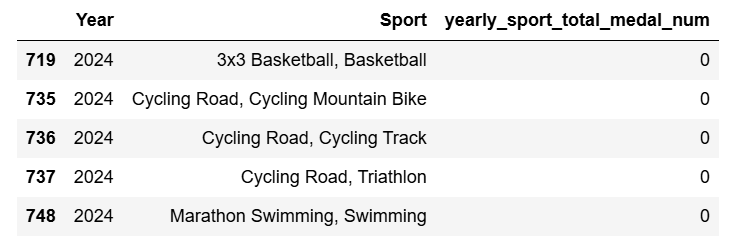
\includegraphics[width=0.8\linewidth]{The statistical situation of the abnormal Sport category.png}
\caption{The statistical situation of the abnormal Sport category} \label{fig1}
\end{figure}

\subsubsection{In "summerOly_programs.csv" file}
\hskip\parindent a) There are encoding issues, suspected to be due to encoding problems, so it was processed using the Windows 1252 encoding. 

b) There are missing values in the programs.csv file. The detailed missing situation is shown in Figure 2.

\begin{figure}[h] 
\centering
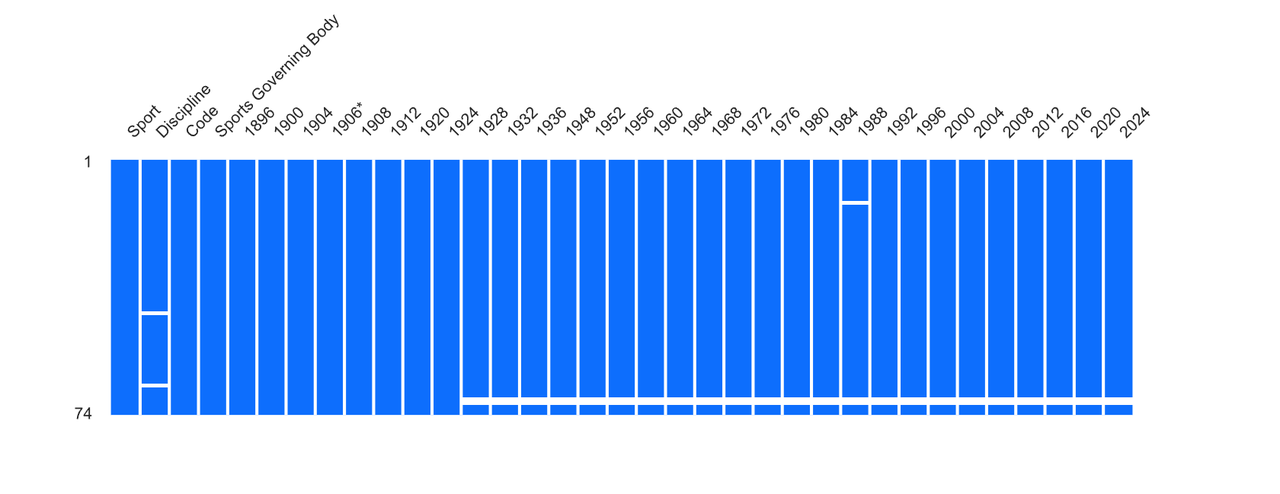
\includegraphics[width=10cm]{Schematic diagram of missing values in the programs table.PNG}
\caption{Schematic diagram of missing values in the programs table} \label{fig1}
\end{figure}
i.The value for 1988 in row 14 is missing.

ii.Figure skating and ice hockey, which are ice sports, were held at the Summer Olympics before 1924. However, they were moved to the first Winter Olympics in 1924, so the values for figure skating and ice hockey in rows 71 and 72 for 1924 and later are missing. 

iii.Because Modern Pentathlon and Water Motorsports do not have further classifications, the “Discipline” values are missing in rows 46 and 67. Based on other data analysis, the “Sport” values of the row was filled into the “Discipline” values. 

\subsubsection{In "summerOly_athletes.csv" and "summerOly_hosts.csv" files}
\hskip\parindent a)Datas for the year {1906} exist in “summerOly_athletes.csv” file but not in the hosts.csv file.

$\bigtriangleup$ Reason: According to research, an unofficial Olympics was held in Athens, Greece, in 1906. 

b)Datas for the years {2028, 2032, 1944, 1940, 1916} exist in “summerOly_hosts.csv” file but not in “summerOly_athletes.csv” file. 

$\bigtriangleup$ Reason: The Olympics for the years {2028, 2032} have not yet taken place. The host countries and cities have been determined, but the participating athletes have not been determined. The three Olympics originally scheduled for the years {1944, 1940, 1916} were canceled due to the two world wars in the 20th century. Although the hosts had been determined, there was no list of participating athletes because they could not be held.

\subsubsection{In "summerOly_medal_counts.csv" file}
\hskip\parindent After reading with UTF-8 encoding, it was found that the 'NOC' column had trailing spaces. All strings in this column were processed to remove excess leading and trailing spaces.

\section{Task 1}

\subsection{Sub-model I:A Multivariate Linear Regression-Based Model for Predicting the Total Medal Count of Countries in the Olympics}

\subsubsection{Model Preparation}
\hskip\parindent From the systematic analysis of influencing factors in the earlier stages, we know that the competitive performance of various countries in the Olympics, specifically quantified as the proportion of the total number of medals won in Olympic competitions, is closely related to the proportion of the total number of events in which the country participates in that year's Olympics. At the same time, the past performance of the country in the Olympics, especially in the previous year and recent years, has a significant and undeniable impact on the total number of medals for the current session.

Based on these factors, let $MP^{i}(t)$ represent the proportion of total medals won by the $i$-th country in the $t$-th Olympics; $S\!-\!Num^{i}(t)$ represents the total number of events participated in by the $i$-th country in the $t$-th Olympics; $P\!-\!Num^{i}(t)$ is the number of medals awarded to athletes from the $i$-th country in the $t$-th Olympic Games; $Home^{i}(t)$is a dummy variable, when the $i$-th country is the host country of the $t$-th Olympics, $Home^{i}(t)=1$, otherwise it equals 0.

\subsubsection{Model Establishment}
\hskip\parindent Because $MP^{i}(t)$ represents the medal-winning rate of each country, it takes values between 0 and 1. We perform a logarithmic transformation on $S\_Num^{i}(t)$ and $P\_Num^{i}(t)$, namely: $S\_Num^{i}(t) = log(S\!-\!Num^{i}(t) + 1)$, $P\_Num^{i}(t) = log(P\!-\!Num^{i}(t) + 1)$.
Thus, it satisfies
\begin{align} \label{eq1}
\notag
MP^{i}(t, \theta) = a_{1}^{i} + a_{2}^{i} \times S\_Num^{i}(t) + a_{3}^{i} \times P\_Num^i(t) \\ 
+ a_{4}^{i} \times Home^{i}(t) + a_{5}^{i} \times MP^{i}(t - 4) + \varepsilon^{i}(t)
\end{align}

Where, $\theta = [a_{1}, a_{2}, a_{3}, a_{4}, a_{5}]$ is the regression coefficient; $t$ is the year of hosting the Olympics; $\varepsilon ^{i}(t)$ encompasses all uncertain factors.

Then we fit it using the least squares method. Let $y^{i}(t)$ be the observed value for the $i$-th country in the $t$-year Olympics. The regression result is $\hat{MP}^{i}(t, \hat{\theta })=\sum_{j=1}^{5}a_{j}^{i}\times f^{i}(t, j)$, and the loss function is $L(\hat{\theta }) = \sum_{t}[y^{i}(t)-\hat{M}^{i}(t, \hat{\theta})]^2$. The parameter estimate that minimizes 
$\hat{\theta }$ is taken as $L(\hat{\theta })$, thus $\hat{MP}^{i}(t, \hat{\theta })$ is the regression outcome.

From the analysis of the above figure, it can be seen that the total count of each Olympic Games shows a linear trend over time. It is noted that data points for the years 1916, 1940, and 1944 are missing, as during these years the Olympics were cancelled due to historical events, thus no records exist. The scatter plot above indicates a generally linear trend. Therefore, we employ a linear function to fit this trend.
\begin{equation}
M\_Sum = \beta_{0} + \beta_{1}t
\end{equation}

Where, $\hat{\beta} = [\beta_{0}, \beta_{1}]$ is the regression coefficient; $t$ refers to the year of the Olympics $-1892$.

We employ OLSE to estimate $\hat{\beta}$, and predict that the total number of medals for the years 2028 and 2032 in Table XXX.

\begin{table}[h]
\centering
\caption{The prediction of the total number of medals.}
\begin{tabular}{|c|c|c|} 
\hline
Year     & ~ 2028~~ & ~ 2032~~  \\ 
\hline
Pre\_Sum & 1026     & 1052      \\
\hline
\end{tabular}
\end{table}

$ Me^{i}(t) = Sum\_M(t)\times MP^{i}(t)$

\subsection{Sub-model II: Exploring the Medal Distribution of Countries Based on Bayesian Models}
\subsubsection{Model Preparation}
\hskip\parindent In the above model construction, we can predict the total medal counts for each country. Let the total number of medals be $N$, with $X$, $Y$, and $Z$ representing the number of gold, silver, and bronze medals respectively, then $N=X+Y+Z$.

(Figure XXX)

If we rank by scoring system, then the total score is $S=W_{1}\times X+W_{2}\times Y+W_{3}\times Z$, with countries scoring higher ranking ahead; if ranked by total medal count, then $S=N$, with countries winning more medals ranking higher.

Based on historical data and experience regarding countries' medal counts, we know that athletes participating in the Olympics can fall into one of four categories: gold medalists, silver medalists, bronze medalists, and those who unfortunately do not win any medals. At the early stages of the competition, we cannot ascertain the true capabilities of participating athletes, thus we can only predict that the probabilities of these four outcomes for each athlete are equal. Similarly, within the total medals awarded to each country, we use a multinomial distribution as the prior distribution, that is 

\begin{equation}
(X, Y, Z|N)\sim Multinomial(N, p_{1}, p_{2}, p_{3})
\end{equation}
 
Where, $p_{1}$, $p_{2}$, and $p_{3}$ are the prior probabilities of gold, silver, and bronze medals, respectively; and $p_{1}+p_{2}+p_{3}=1$.
\begin{figure}[h] 
\centering
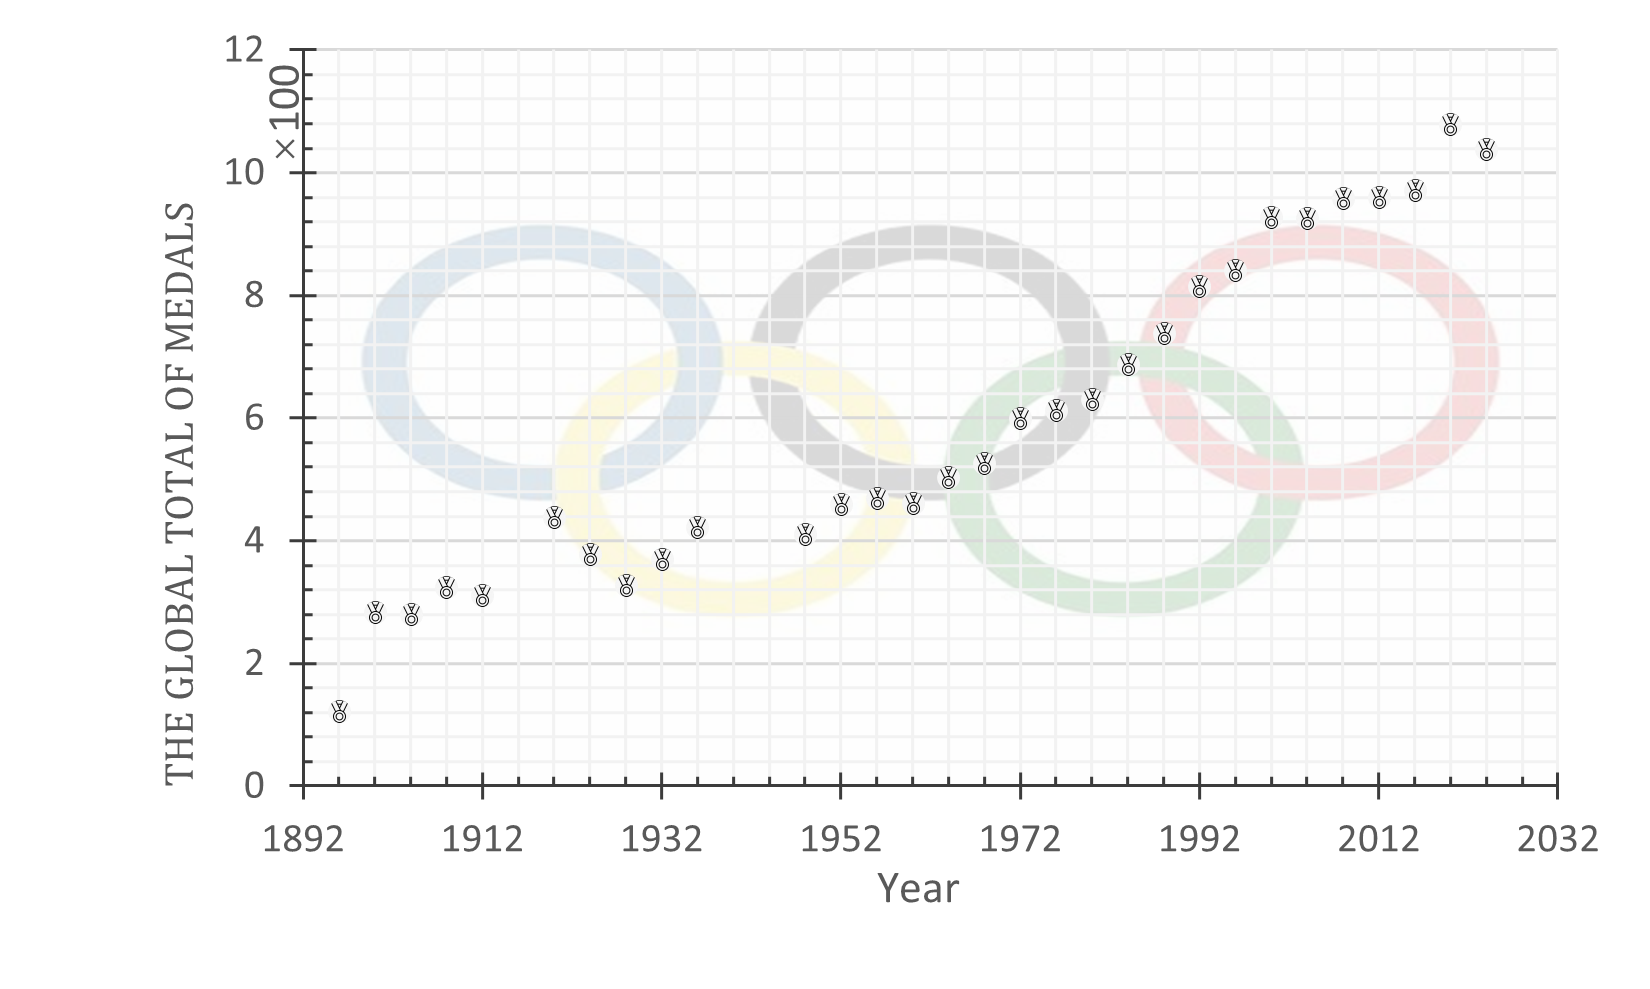
\includegraphics[width=10cm]{Global Total Olympic Medals Over Time.png}
\caption{Global Total Olympic Medals Over Time}
\end{figure}

\subsubsection{Model Establishment}
\hskip\parindent Based on the specific medal counts of various countries, $D^i(t)={X^{i}(t), Y^{i}(t), Z^{i}(t)}$ represents the number of gold, silver, and bronze medals country $i$ wins in $t$ year.

Here, $i\in \{France, United States, Germany, Australia, ...\}$, $t\in \{1896, 1900, ...,2024\}$.

Assuming the observations for year $t$ from country $i$ are independent and identically distributed given the winning situation, the sample likelihood function can be expressed as $P(D^{i}|X^{i}, Y^{i}, Z^{i})= \prod_{t}(p(x^{i}(t), y^{i}(t), z^{i}(t)|X, Y, Z)$.

Under the assumption of a multinomial prior distribution, for every group of historical sample data, $(x^{i}(t), y^{i}(t), z^{i}(t))$, its probability distribution can be expressed as $P(x^{i}(t), y^{i}(t), z^{i}(t)|N)=\frac{N!}{x^{i}!y^{i}!z^{i}!}P_{1} ^{x^{i}}P_{2} ^ {y^{i}}P_{3} ^ {z^{i}}$, thus the likelihood function is $P(D|X, Y, Z)=\prod_{i=1}^{n}\frac{N!}{x^{i}!y^{i}!z^{i}!}P_{1}^{x^{i}}P_{2}^{y^{i}}P_{3}^{z^{i}}$.

Substituting the prior distribution and the likelihood function into the equation, and computing the normalization constant C ensures that $\sum_{x+y+z=N}P(X=x, Y=y, Z=z|D)=1$.

Thus, the posterior distribution can be expressed as: $P(X^{i}(t), Y^{i}(t), Z^{i}(t)|D) = \frac{1}{c} \times \frac{N!}{x!y!z!}P_{1}^{x}P_{2}^{y}P_{3}^{z}\prod_{t=1}^{n}\frac{N!}{x^{i}(t)!y^{i}(t)!z^{i}(t)!}P_{1}^{x^{i}(t)}P_{2}^{y^{i}(t)}P_{3}^{z^{i}(t)}$.

By introducing the Bayesian model, in combination with the prior distribution and historical data, we can effectively evaluate the number of gold medals won given the total number of medals is known.

\subsection{Model Improvement Based on Advantage Project Relaxation Function}
As the medal count does not adequately measure the ability of athletes from countries that have never won any medals, we modify the multiple linear regression model. In this case, the assessment of athletes' capabilities from a country is not only based on the total count of medals won but also considers all data regarding the events and awards of athletes provided in the data set, including results from unofficial competitions. Thus, we adjust the independent variable $P\_Num^{i}(t)$ to ensure $P_{1}\_Num^{i}(t) = P+P\_Num^{i}(t)$, where $P$ indicates the minimum level of the country's athletes, measured by the participation rate in events from that country. Additionally, the effect of project advantages also influences the medal-winning outcomes of countries to some extent. By considering the number and types of events, we adjust the independent variable $S\_Num^{i}(t)$ as follows:
\begin{equation}
S_{1}\_Num^{i}(t) = S\_Num^{i}(t) + f(p)
\end{equation}

Where, $f(p) = \sum_{k=1}^{n}w_{k}I_{k}$ and $w_{k}$ represent the weight proportions for various projects; $I_{k}$ represents the count variable for project types.

Therefore, the modified multiple linear regression function is $MP^{i}(t, \theta) = a_{1}^{i}+a_{2}^{i}\times S_{1}\_Num^{i}(t) + a_{3}^{i}\times P_{1}\_Num^{i}(t) + a_{4}^{i}\times H^{i}(t) + a_{5}^{i}MP^{i}(t-4)$.

Since the previously mentioned random variables $X^{i}(t)$, $Y^{i}(t)$, and $Z^{i}(t)$ do not constitute a completely independent variation process in practice, their random fluctuations and magnitudes are influenced by the types and number of events that the country participates in, thus the values of $P_{1}^{i}(t)$, $P_{2}^{i}(t)$, and $P_{3}^{i}(t)$ will change with the number and type of events, as categorized below:

\begin{equation}
Item_{i, j}(t) = \frac{M_{i, j}(t)}{S_{i, j}(t)} \times \frac{P\_Num^{i}(t)}{S\_Num^{i}(t)}
\end{equation}

Advantage Projects: ???
Balanced Projects:???
Disadvantage Projects:???

\begin{figure}[h] 
\centering
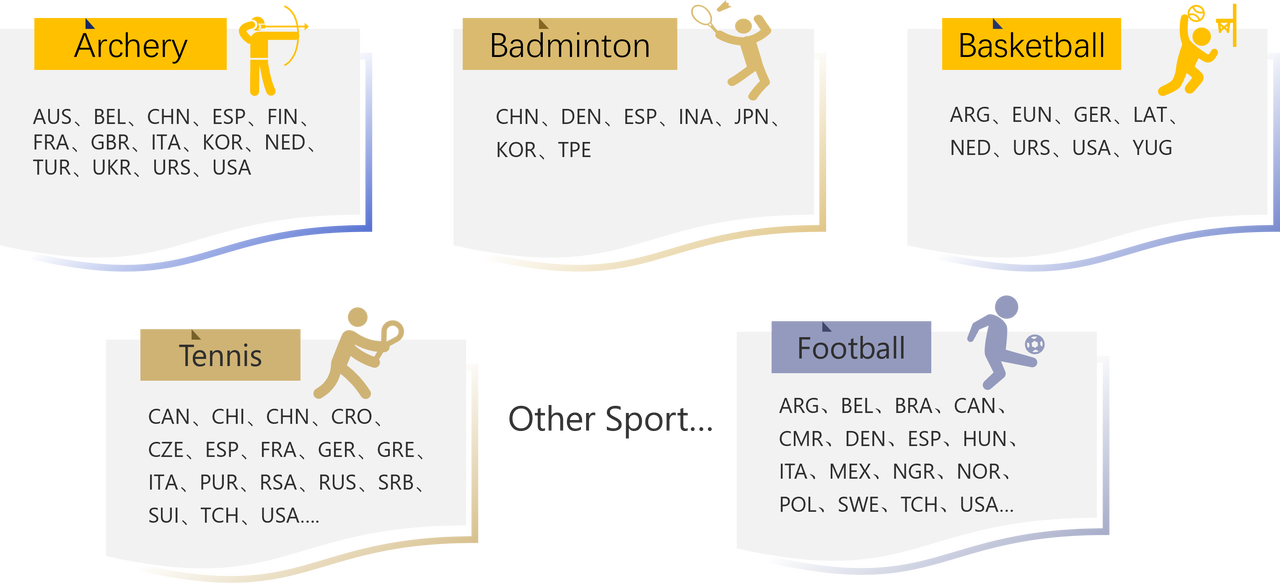
\includegraphics[width=10cm]{Advantageous projects and corresponding countries.png}
\caption{Advantageous projects and corresponding countries}
\end{figure}


In this thesis, we observe that when a project is an advantage project for the country, there is a higher likelihood of winning gold medals, while performance in non-advantage projects is less optimistic. Therefore, we introduce an advantage project relaxation function $f(M)$ to correct the Bayesian model $P_{j}^{oi}(t) = P_{j}^{i}(t)f(M)$.

Thus, the revised Bayesian estimation is:
$P_{1}^{o}$

$P_{1}$

$Me^{i}\times P_{1}^{oi}$

This allows us to estimate the value of p1 through Bayesian estimation, ultimately predicting the number of gold medals won by various countries to be (variable XXX).

\begin{table}
\centering
\caption{ The prediction of the award situations in 2028}
\begin{tabular}{ccc|ccc} 
\hline
\multicolumn{3}{c|}{Top 10}         & \multicolumn{3}{c}{Bottom 10}            \\ 
\hline
Country      & ~ rank~~ & ~ Medal~~ & ~ ~ ~Country~ ~~ & ~ rank~~ & ~ Medal~~  \\ 
\hline
UnitedStates & 1        & 106       & Hungary          & 11       & 23         \\
China        & 2        & 87        & Cuba             & 12       & 22         \\
GreatBritain & 3        & 82        & Canada           & 13       & 20         \\
Germany      & 4        & 59        & Ukraine          & 14       & 19         \\
Australia    & 5        & 47        & Brazil           & 15       & 18         \\
Italy        & 6        & 42        & Spain            & 16       & 18         \\
Japan        & 7        & 42        & Sweden           & 17       & 16         \\
SouthKorea   & 8        & 35        & Kenya            & 18       & 15         \\
Netherlands  & 9        & 27        & Norway           & 19       & 15         \\
France       & 10       & 23        & Poland           & 20       & 15         \\
\hline
\end{tabular}
\end{table}

\subsection{Uncertainty analysis of the influence model}
$e^{i}$

$MP^{i}_{j}$

$\hat{MP}^{i}_{j}$

\begin{equation}
e^{i}_{j} = MP^{i}_{j}-\hat{MP}^{i}_{j}
\end{equation}

$E(e^{i}_j) = 0$

\begin{figure}[htbp]
	\centering
	\begin{minipage}{0.4\linewidth}
		\centering
		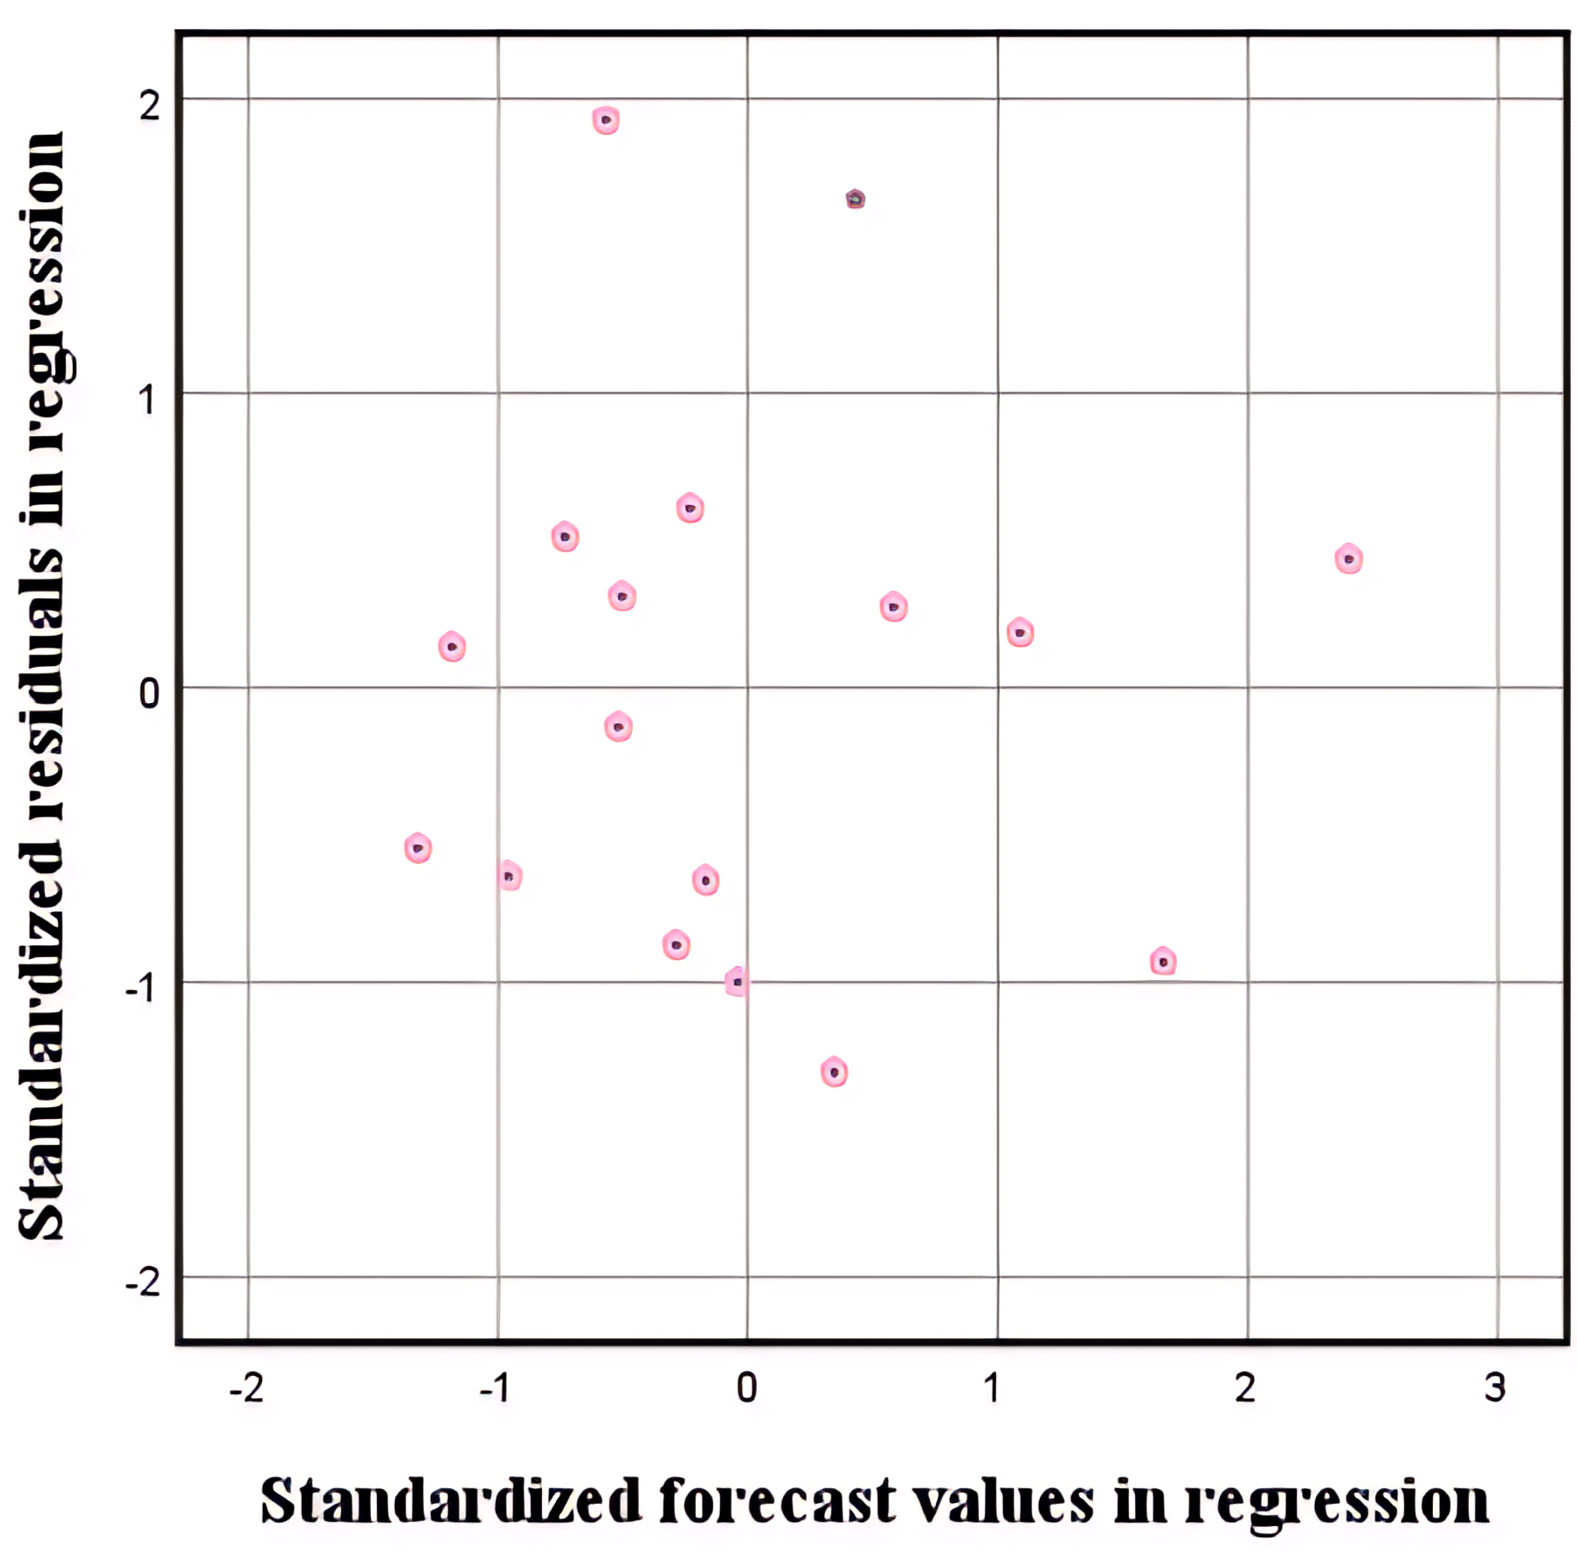
\includegraphics[width=1\linewidth]{Residual plot.png}
		\caption{Residual plot}
	\end{minipage}
	\begin{minipage}{0.4\linewidth}
		\centering
		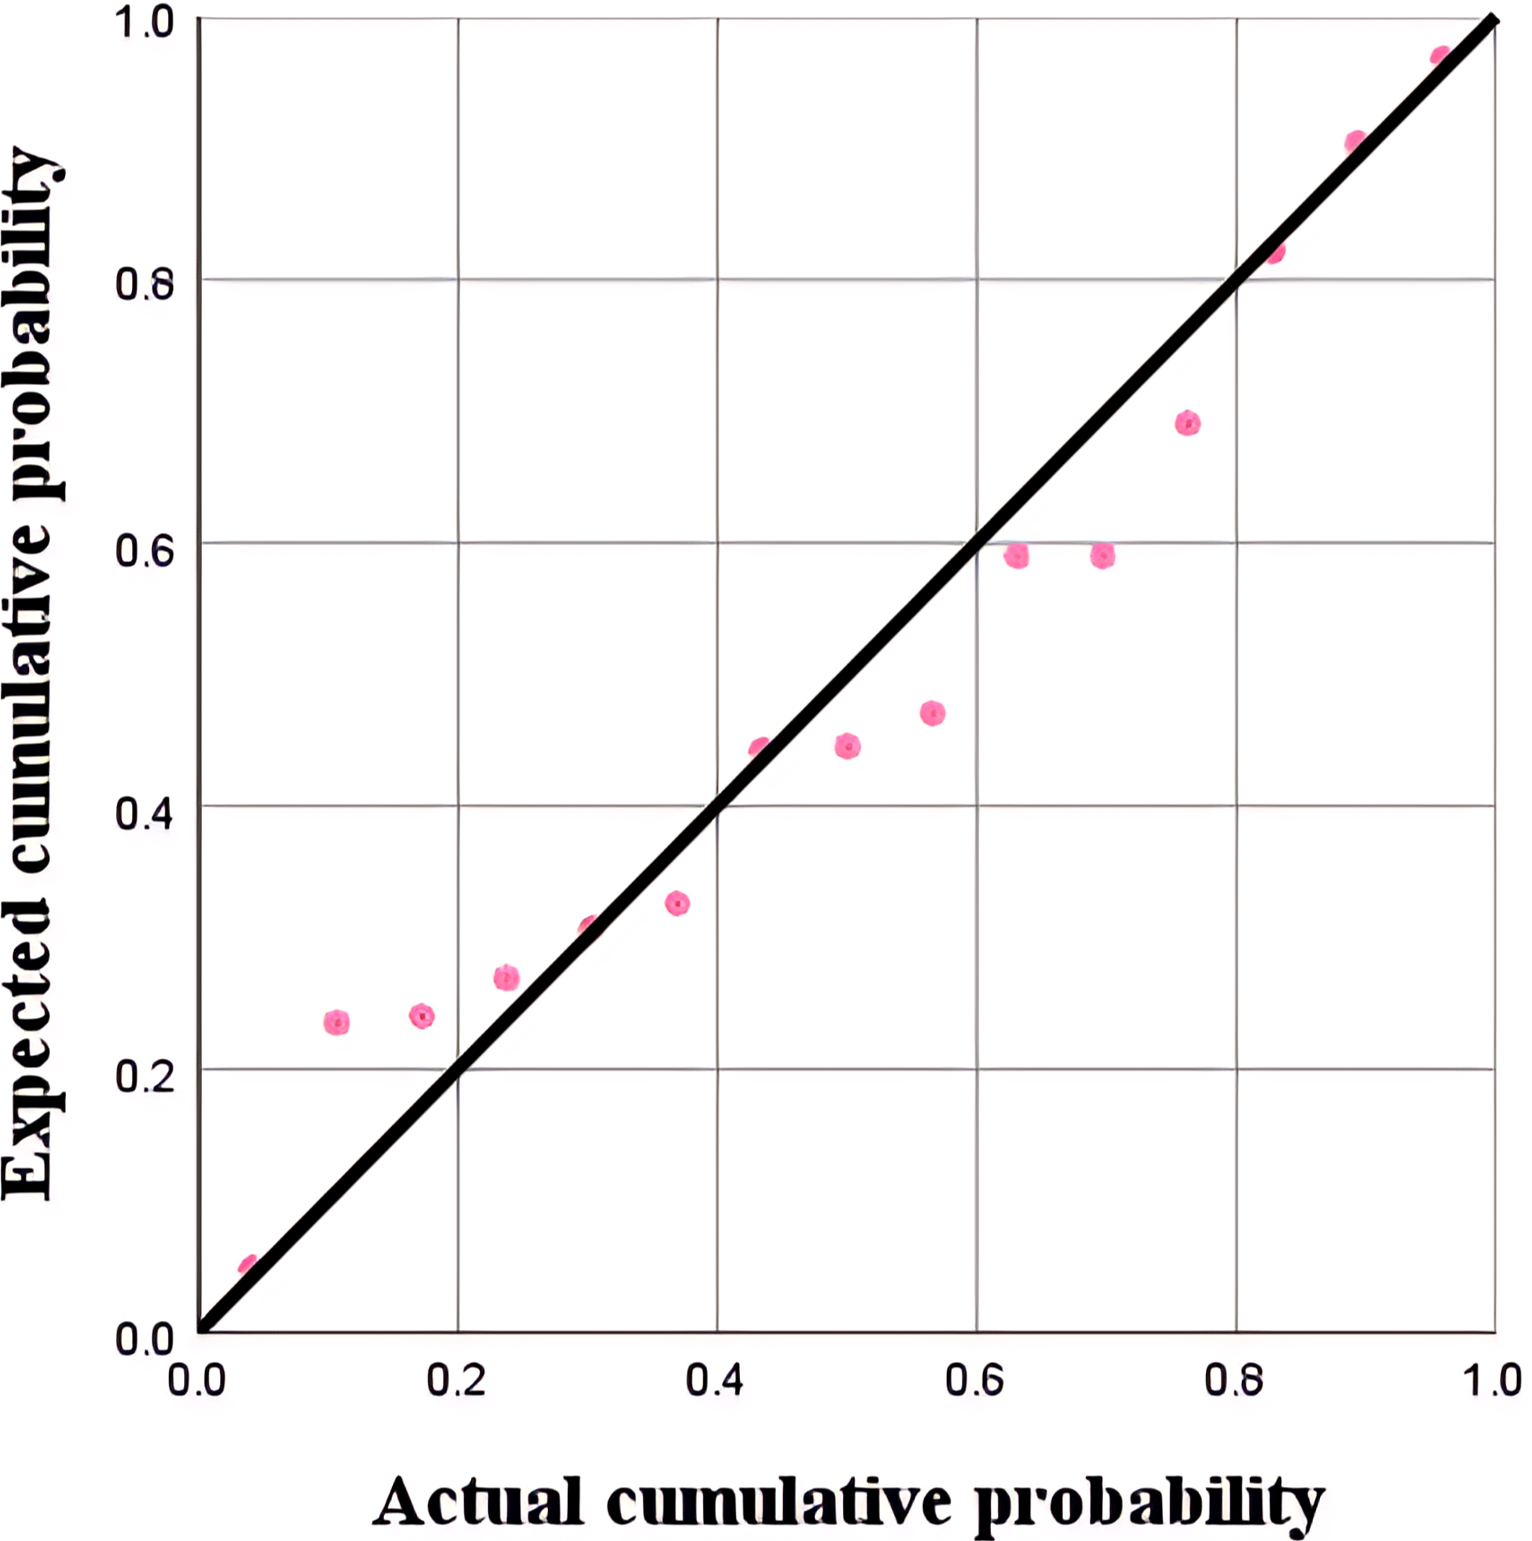
\includegraphics[width=1\linewidth]{Quantile-Quantile Plot.png}
		\caption{Quantile-Quantile plot}
	\end{minipage}
\end{figure}

\subsection{Revealing the results of the medal table for future Olympic Games}

\begin{table}
\centering
\caption{Regression coefficient of the trend prediction model}
\begin{tabular}{|c|c|c|c|c|c|c|} 
\hline
\multirow{2}{*}{Country} & \multicolumn{5}{c|}{$\theta$}               & \multirow{2}{*}{$R^{2}$}  \\ 
\cline{2-6}
                         & a1    & a2    & a3    & a4    & a5    &                    \\ 
\hline
Australia                & 0.023 & 0.141 & 0.190 & 0.351 & 0.281 & 0.877              \\ 
\hline
Belarus                  & 0.011 & 0.054 & 0.113 & 0.000 & 0.764 & 0.769              \\ 
\hline
Belgium                  & 0.124 & 0.314 & 0.215 & 0.241 & 0.465 & 0.864              \\ 
\hline
China                    & 0.141 & 0.521 & 0.121 & 0.327 & 0.684 & 0.880              \\ 
\hline
United States            & 0.118 & 0.381 & 0.241 & 0.261 & 0.763 & 0.792              \\
\hline
\end{tabular}
\end{table}


\begin{table}
\centering
\caption{Prediction interval for the number of Medalsa in difference Country}
\arrayrulecolor[rgb]{1,0.482,0}
\begin{tabular}{|c|ccc|} 
\hhline{|----|}
\rowcolor[rgb]{1,0.482,0} \multicolumn{1}{|c}{{\cellcolor[rgb]{1,0.482,0}}}                                      & {\cellcolor[rgb]{1,0.482,0}}                                    & \multicolumn{2}{c|}{~ ~Confidence interval of 0.95~ ~}                             \\
\rowcolor[rgb]{1,0.482,0} \multicolumn{1}{|c}{\multirow{-2}{*}{{\cellcolor[rgb]{1,0.482,0}}~ ~ ~ Country~ ~ ~~}} & \multirow{-2}{*}{{\cellcolor[rgb]{1,0.482,0}}~ ~ Pre\_2028~ ~~} & {\cellcolor[rgb]{1,0.824,0.635}}LMCI\_2 & {\cellcolor[rgb]{1,0.824,0.635}}UMCI\_2  \\ 
\hline
{\cellcolor[rgb]{0.992,0.737,0.529}}United States                                                                & 106                                                             & 94                                      & 134                                      \\ 
\hline
\rowcolor[rgb]{1,0.824,0.635} {\cellcolor[rgb]{0.992,0.737,0.529}}China                                          & 87                                                              & 72                                      & 102                                      \\ 
\hline
{\cellcolor[rgb]{0.992,0.737,0.529}}GreatBritain                                                                 & 82                                                              & 41                                      & 123                                      \\ 
\hline
\rowcolor[rgb]{1,0.824,0.635} {\cellcolor[rgb]{0.992,0.737,0.529}}Germany                                        & 59                                                              & 37                                      & 80                                       \\ 
\hline
{\cellcolor[rgb]{0.992,0.737,0.529}}Australia                                                                    & 47                                                              & 37                                      & 57                                       \\ 
\hline
\rowcolor[rgb]{1,0.824,0.635} {\cellcolor[rgb]{0.992,0.737,0.529}}Italy                                          & 42                                                              & 30                                      & 55                                       \\ 
\hline
{\cellcolor[rgb]{0.992,0.737,0.529}}Japan                                                                        & 42                                                              & 33                                      & 51                                       \\ 
\hline
\rowcolor[rgb]{1,0.824,0.635} {\cellcolor[rgb]{0.992,0.737,0.529}}SouthKorea                                     & 35                                                              & 22                                      & 48                                       \\ 
\hline
{\cellcolor[rgb]{0.992,0.737,0.529}}Netherlands                                                                  & 27                                                              & 19                                      & 36                                       \\ 
\hline
\rowcolor[rgb]{1,0.824,0.635} {\cellcolor[rgb]{0.992,0.737,0.529}}France                                         & 23                                                              & -4                                      & 51                                       \\ 
\hline
{\cellcolor[rgb]{0.992,0.737,0.529}}Hungary                                                                      & 23                                                              & 15                                      & 32                                       \\ 
\hline
\rowcolor[rgb]{1,0.824,0.635} {\cellcolor[rgb]{0.992,0.737,0.529}}Cuba                                           & 22                                                              & 13                                      & 32                                       \\ 
\hline
{\cellcolor[rgb]{0.992,0.737,0.529}}Canada                                                                       & 20                                                              & 12                                      & 28                                       \\ 
\hline
\rowcolor[rgb]{1,0.824,0.635} {\cellcolor[rgb]{0.992,0.737,0.529}}Ukraine                                        & 19                                                              & 4                                       & 33                                       \\ 
\hline
{\cellcolor[rgb]{0.992,0.737,0.529}}Brazil                                                                       & 18                                                              & 15                                      & 22                                       \\ 
\hline
\rowcolor[rgb]{1,0.824,0.635} {\cellcolor[rgb]{0.992,0.737,0.529}}Spain                                          & 18                                                              & 5                                       & 31                                       \\ 
\hline
{\cellcolor[rgb]{0.992,0.737,0.529}}Sweden                                                                       & 16                                                              & 7                                       & 26                                       \\ 
\hline
\rowcolor[rgb]{1,0.824,0.635} {\cellcolor[rgb]{0.992,0.737,0.529}}Kenya                                          & 15                                                              & 9                                       & 21                                       \\ 
\hline
{\cellcolor[rgb]{0.992,0.737,0.529}}Norway                                                                       & 15                                                              & 8                                       & 21                                       \\ 
\hline
\rowcolor[rgb]{1,0.824,0.635} {\cellcolor[rgb]{0.992,0.737,0.529}}Poland                                         & 15                                                              & 8                                       & 22                                       \\
\hline
\end{tabular}
\arrayrulecolor{black}
\end{table}

\begin{figure}[h] 
\centering
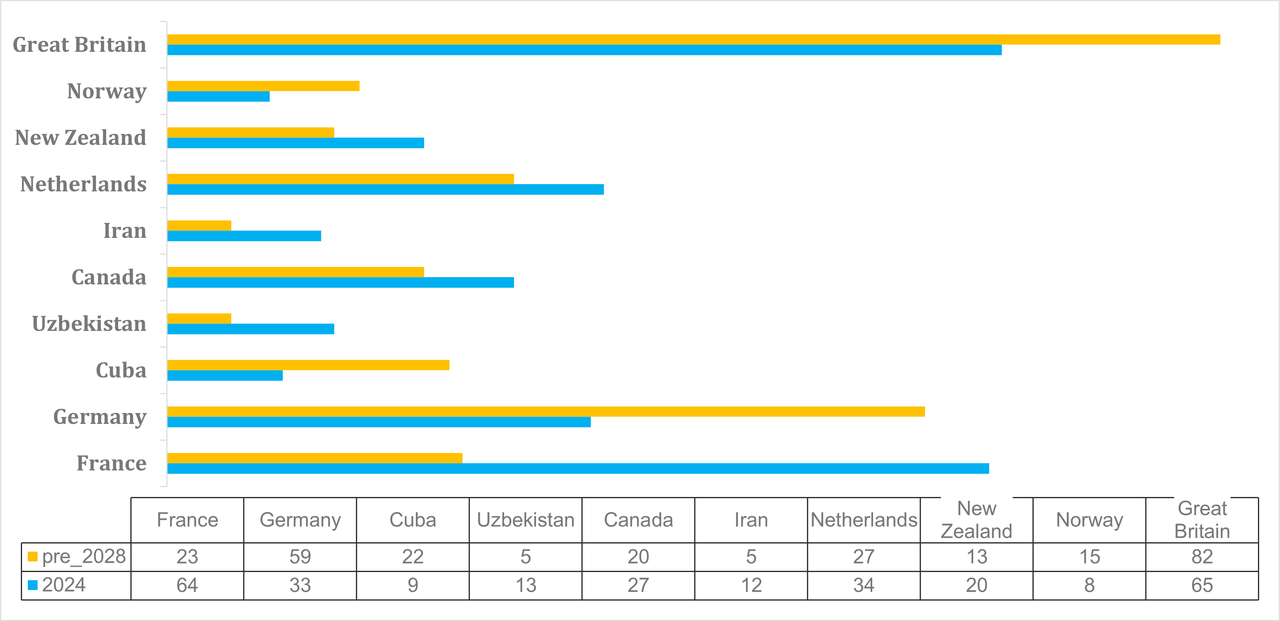
\includegraphics[width=10cm]{Chart of the Medal Counts Changes of the Top 10 Countries.png}
\caption{Chart of the Medal Counts Changes of the Top 10 Countries}
\end{figure}

\begin{figure}[h] 
\centering
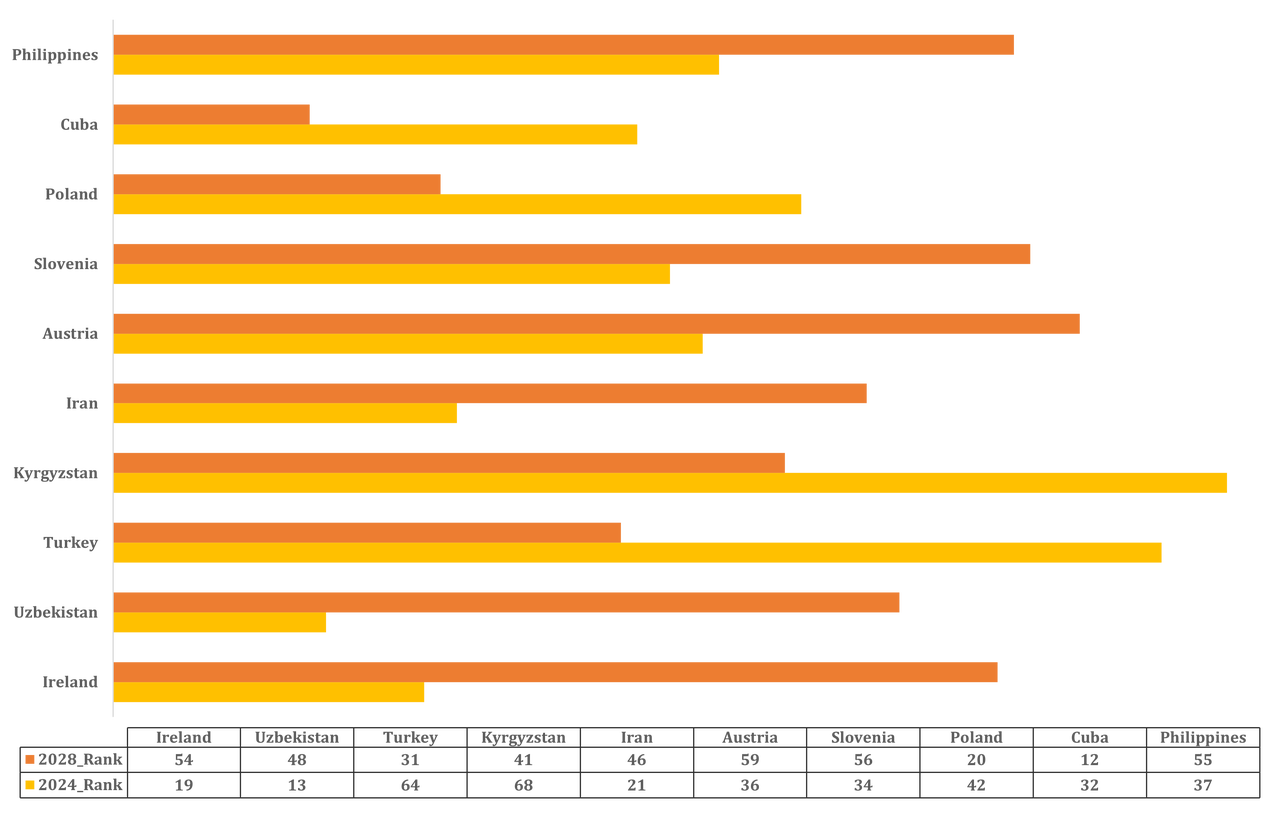
\includegraphics[width=10cm]{Chart for Comparing the Ranking Changes of the Top 10 Countries.png}
\caption{Chart for Comparing the Ranking Changes of the Top 10 Countries}
\end{figure}

\begin{table}
\centering
\caption{Table of the Countries Achieving Zero-breakthrough and  Probabilities}
\begin{tabular}{|c|c|c|c|} 
\hline
\textbf{~ ~ ~ Country~ ~ ~~} & \textbf{~ Probability~~} & \textbf{Country}                 & \textbf{~ Probability~~}  \\ 
\hline
Nicaragua                    & 0.129217                 & Tuvalu                           & 0.131417                  \\ 
\hline
Libya                        & 0.112495                 & South Sudan                      & 0.118437                  \\ 
\hline
Comoros                      & 0.144345                 & Lebanon                          & 0.131196                  \\ 
\hline
Malawi                       & 0.130465                 & Democratic Republic of the Congo & 0.145907                  \\ 
\hline
Rhodesia                     & 0.131206                 & East Timor                       & 0.102365                  \\ 
\hline
Cook Islands                 & 0.100384                 & Eswatini                         & 0.097714                  \\ 
\hline
Peri                         & 0.137529                 & St Kitts and Nevis               & 0.116556                  \\ 
\hline
South Vietnam                & 0.140657                 & StVincentGrenadines              & 0.122315                  \\ 
\hline
Cambodia                     & 0.148522                 & Timor-Leste                      & 0.13819                   \\ 
\hline
Kingfisher                   & 0.117098                 & Brunei Darussalam                & 0.097726                  \\ 
\hline
Yangon                       & 0.129572                 & DR Congo                         & 0.120408                  \\
\hline
\end{tabular}
\end{table}

$p_{1}$

$Me^{i}\times p_{1}^{i}$

\begin{figure}[htbp]
	\centering
	\begin{minipage}{0.4\linewidth}
		\centering
		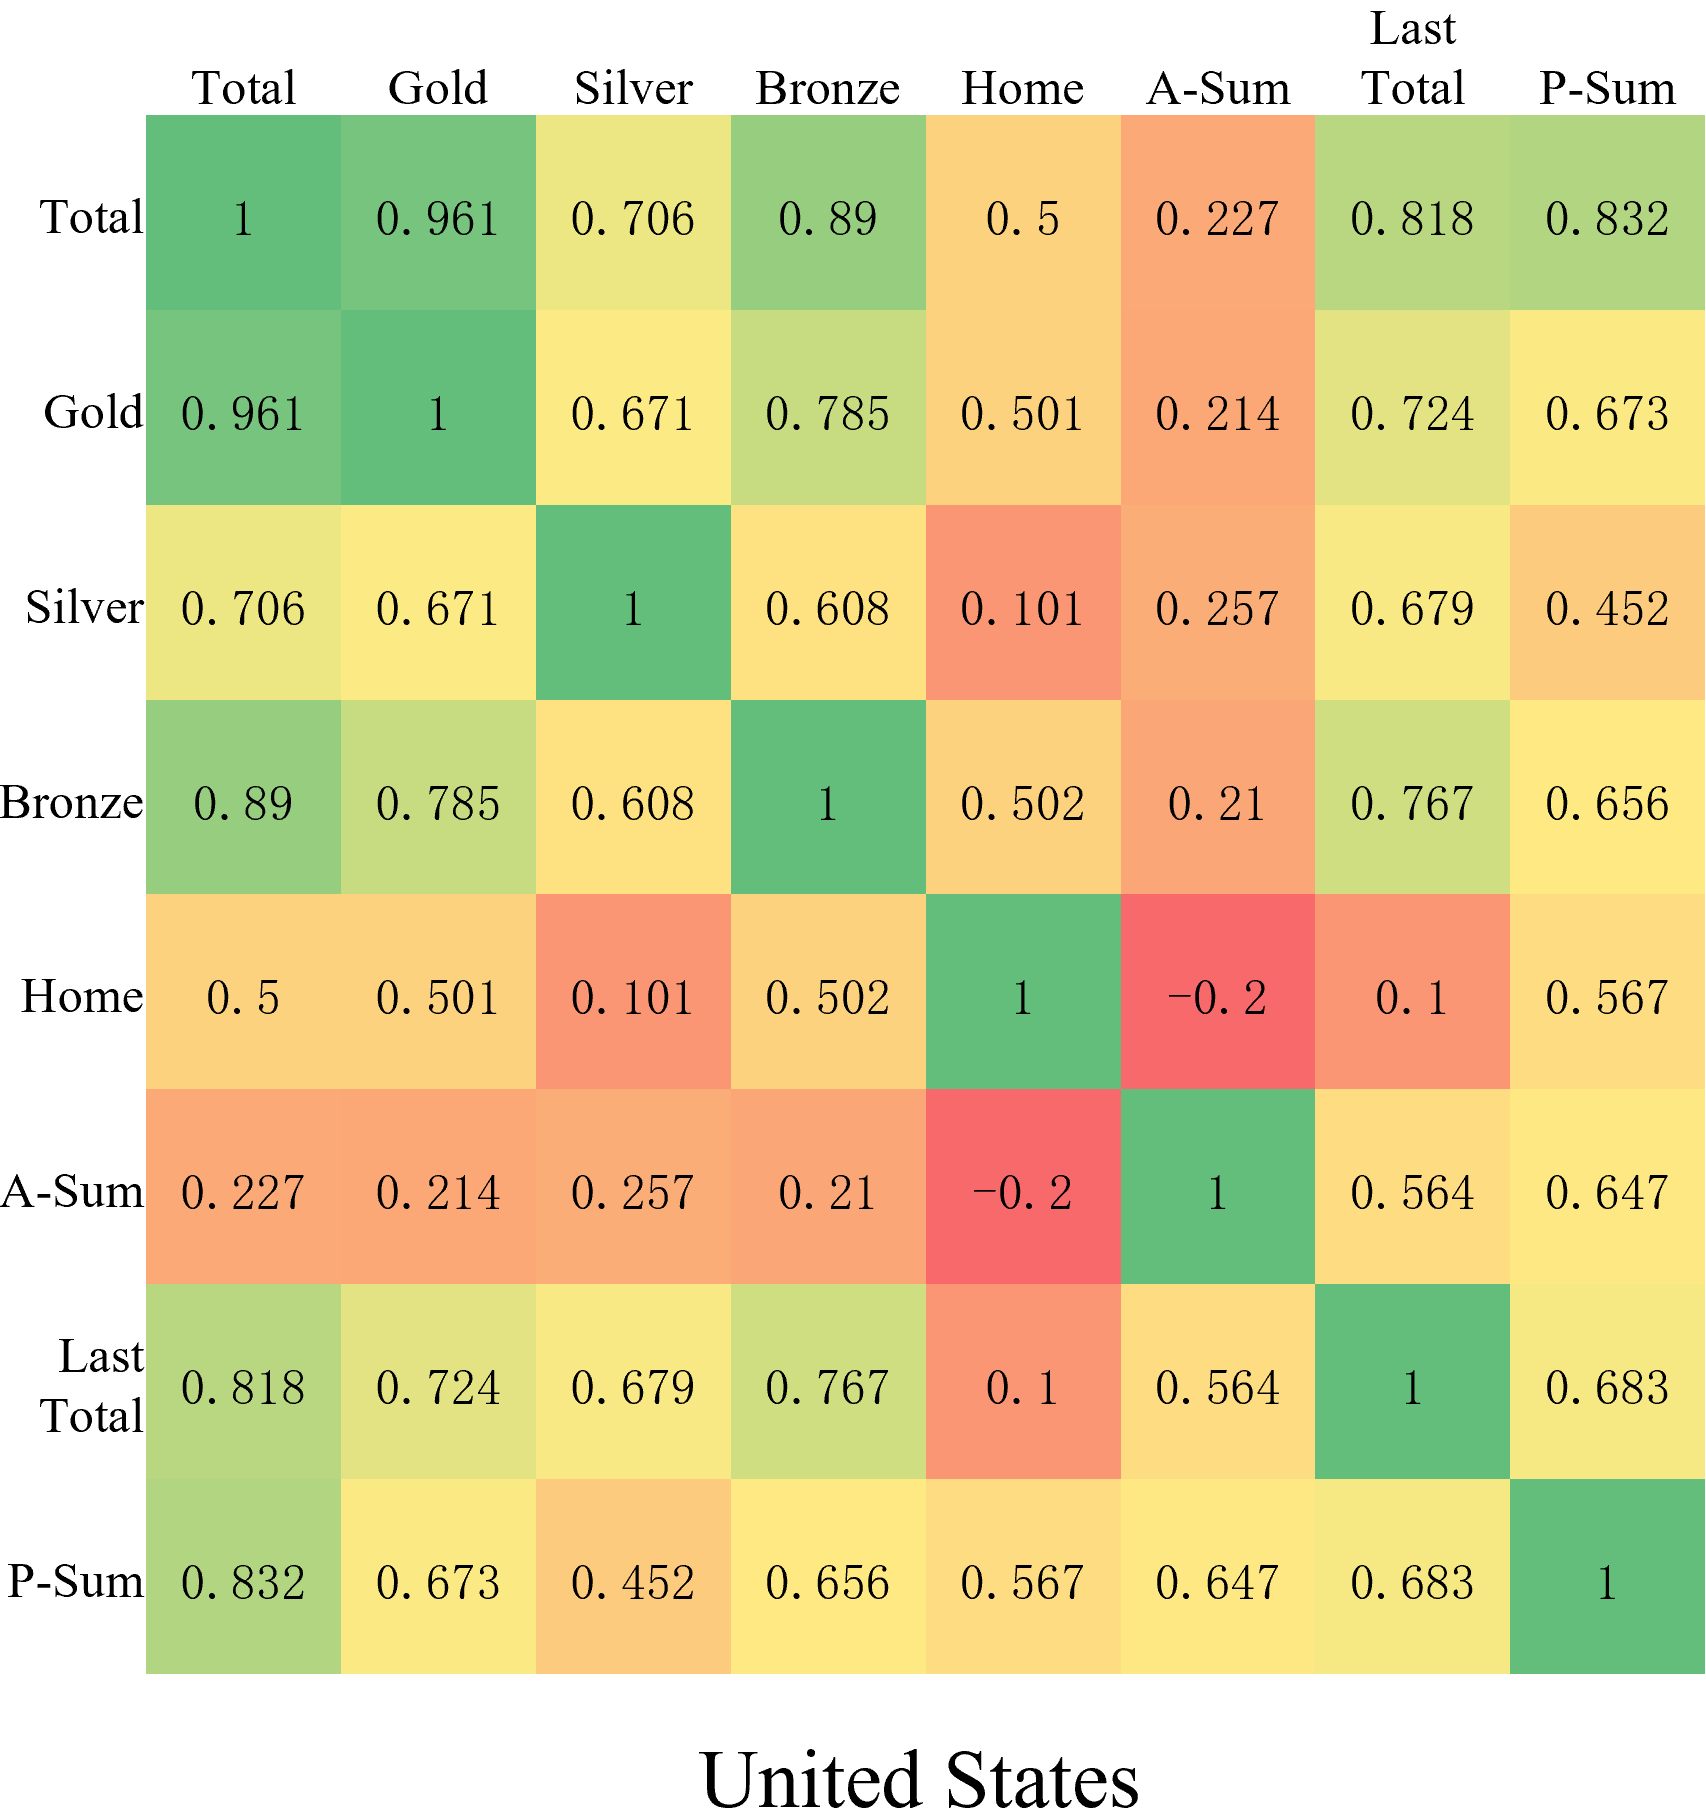
\includegraphics[width=1\linewidth]{Some_figures_1.png}
	\end{minipage}
	\begin{minipage}{0.4\linewidth}
		\centering
		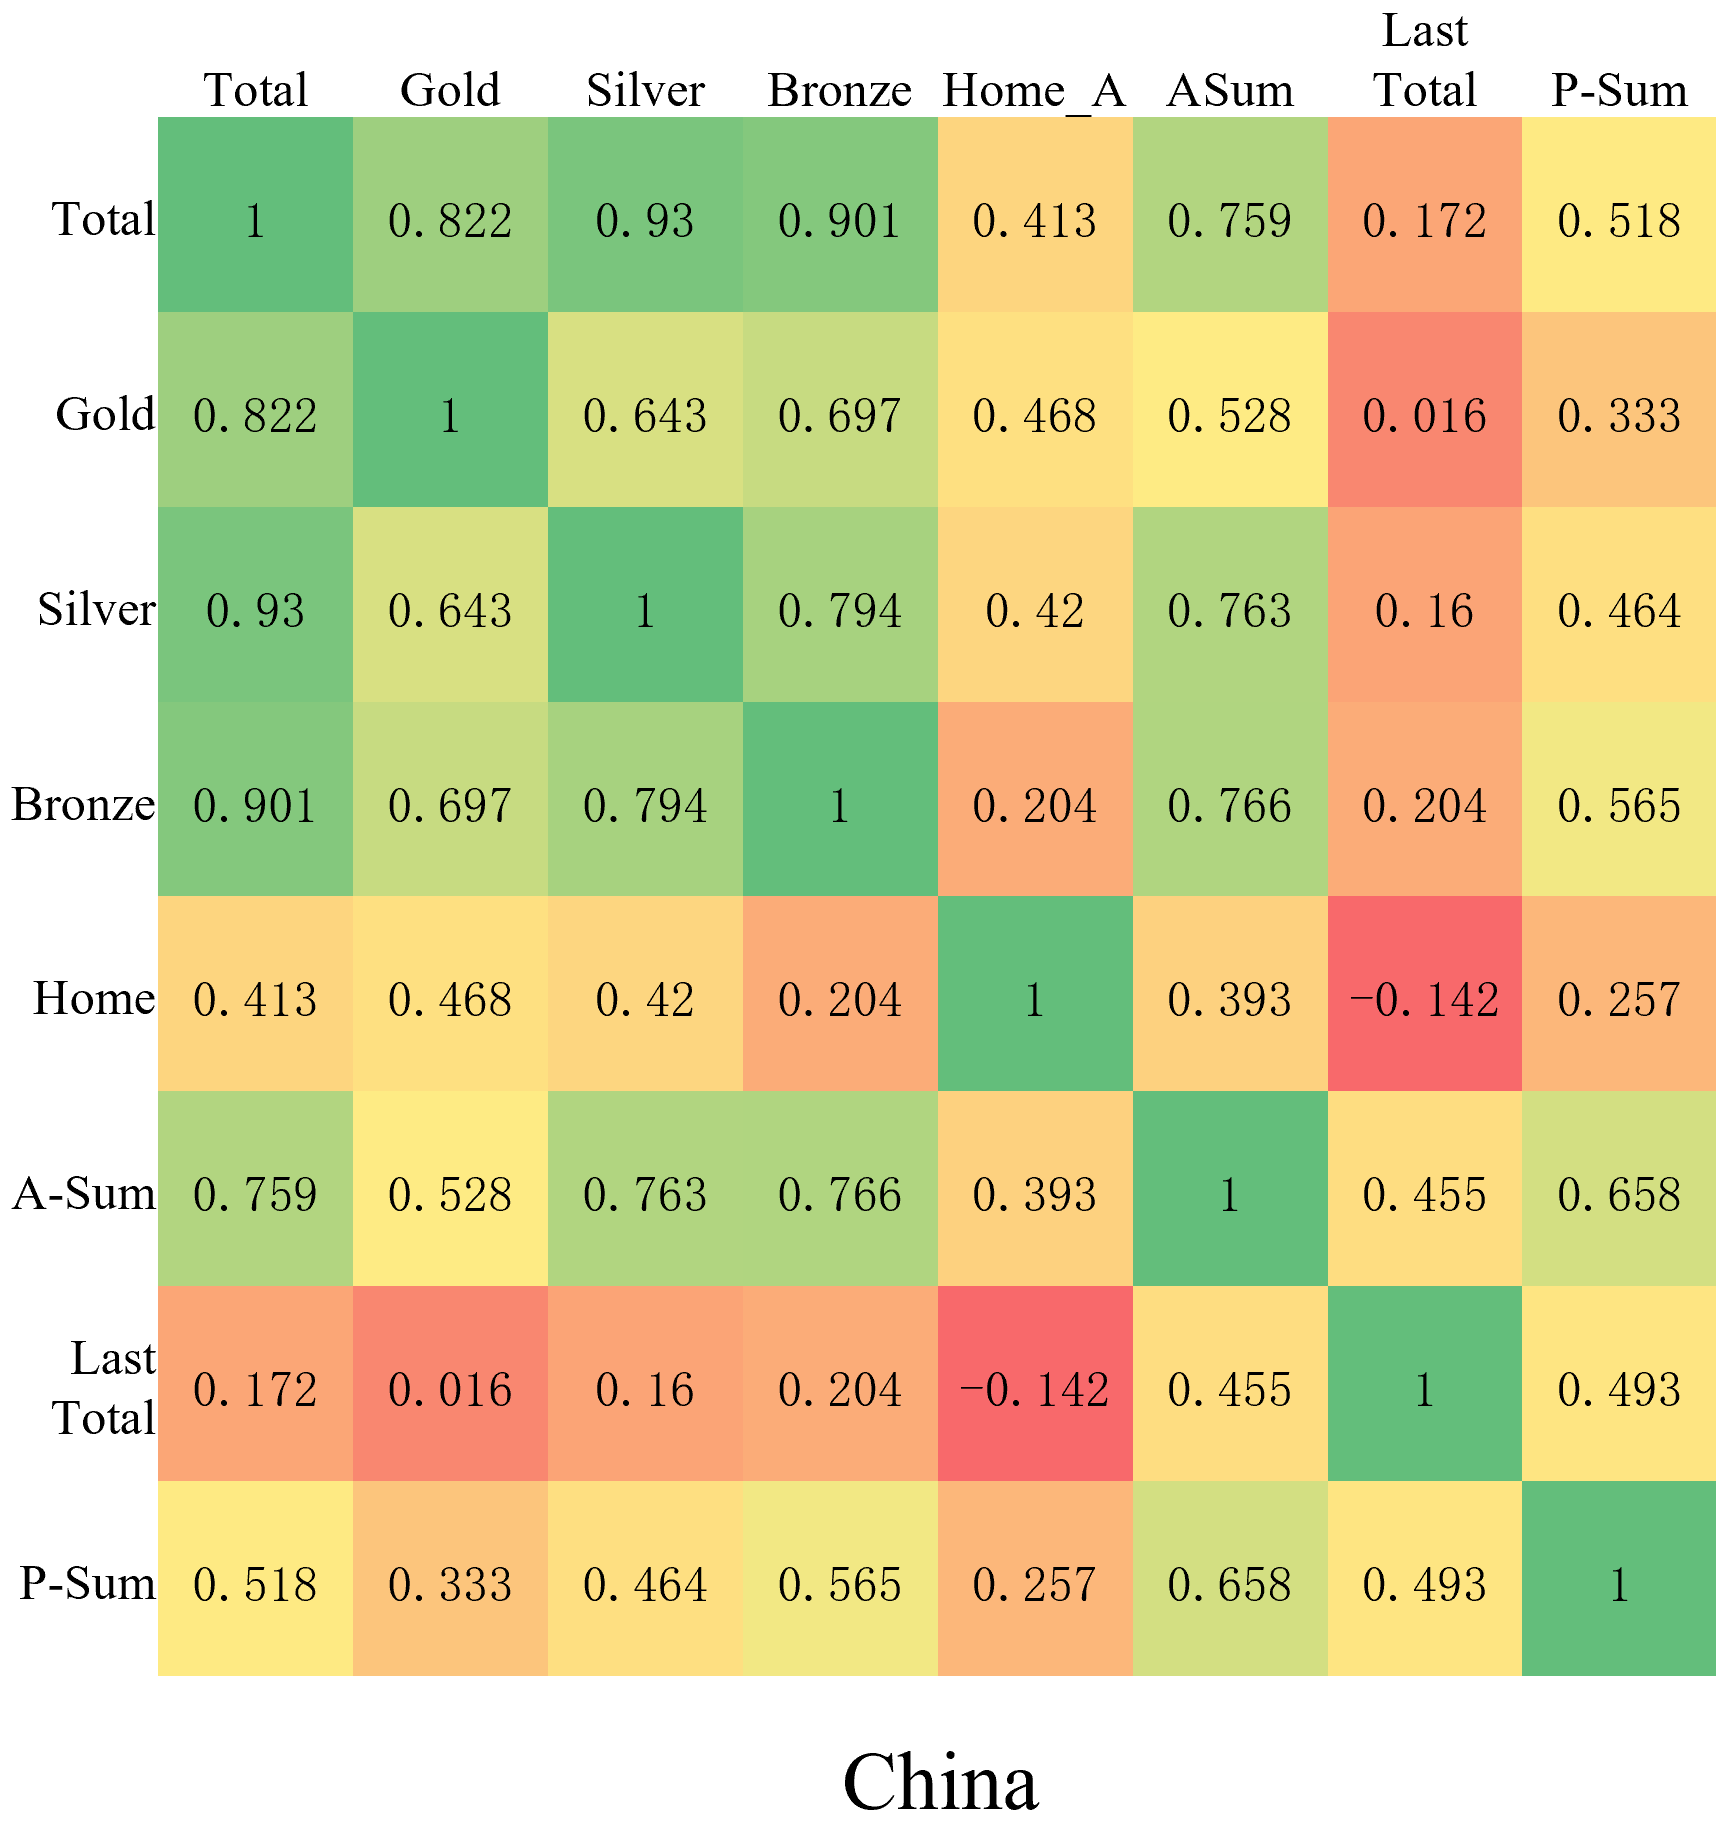
\includegraphics[width=1\linewidth]{Some_figures_2.png}
	\end{minipage}
	\begin{minipage}{0.4\linewidth}
		\centering
		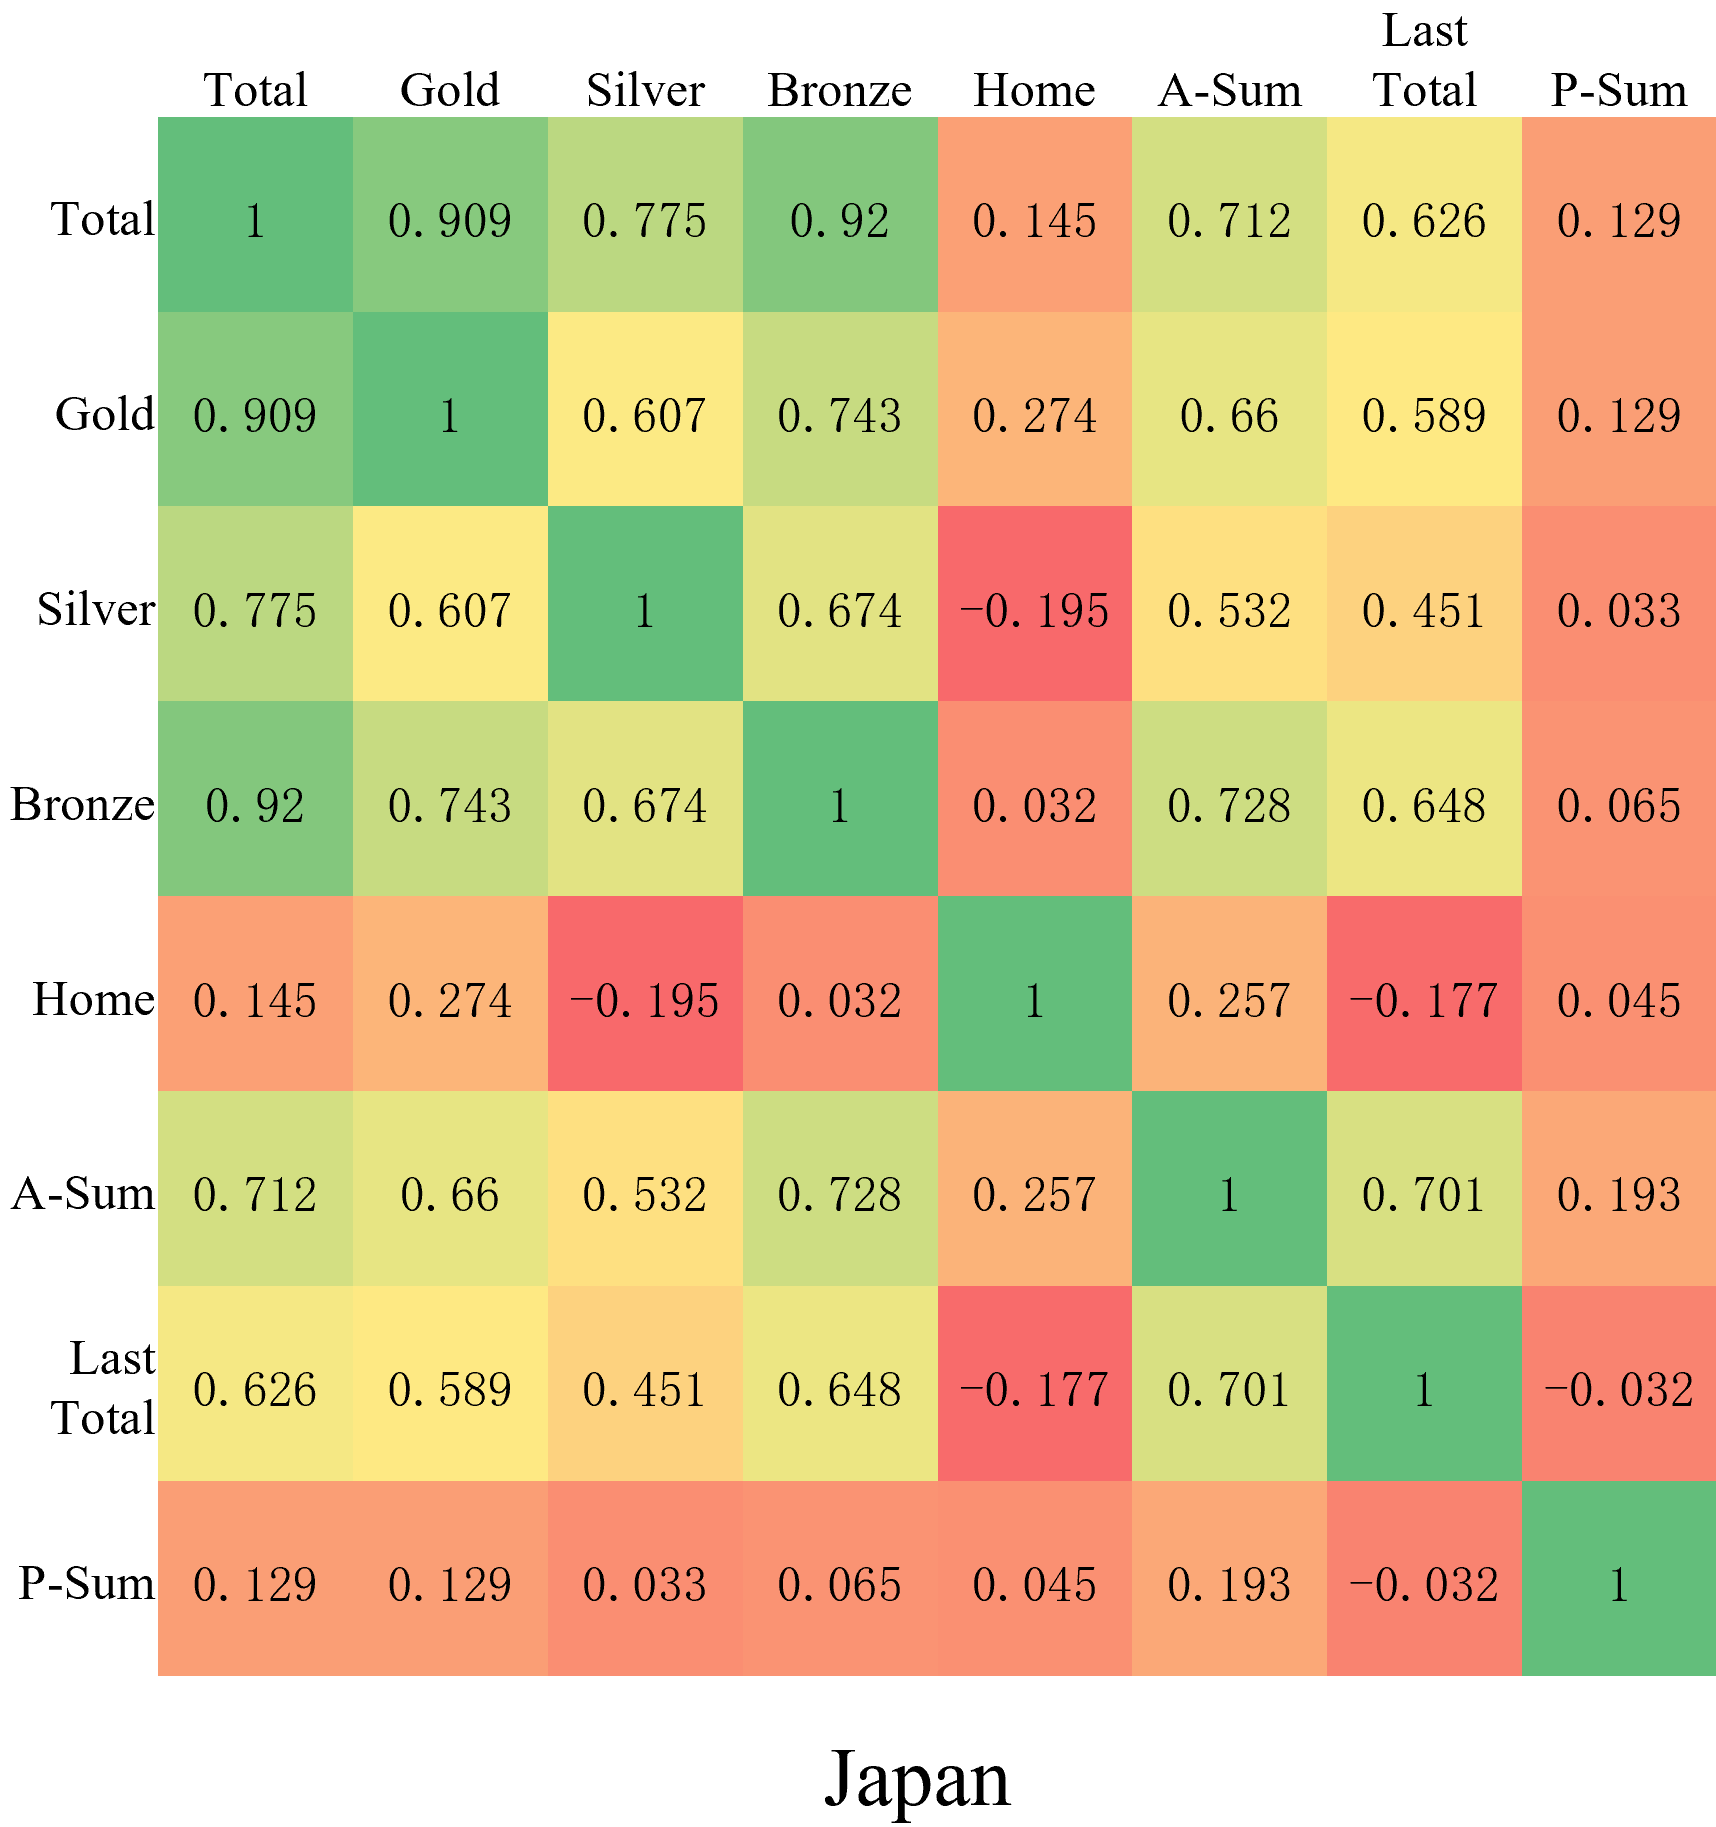
\includegraphics[width=1\linewidth]{Some_figures_3.png}
	\end{minipage}
	\begin{minipage}{0.4\linewidth}
		\centering
		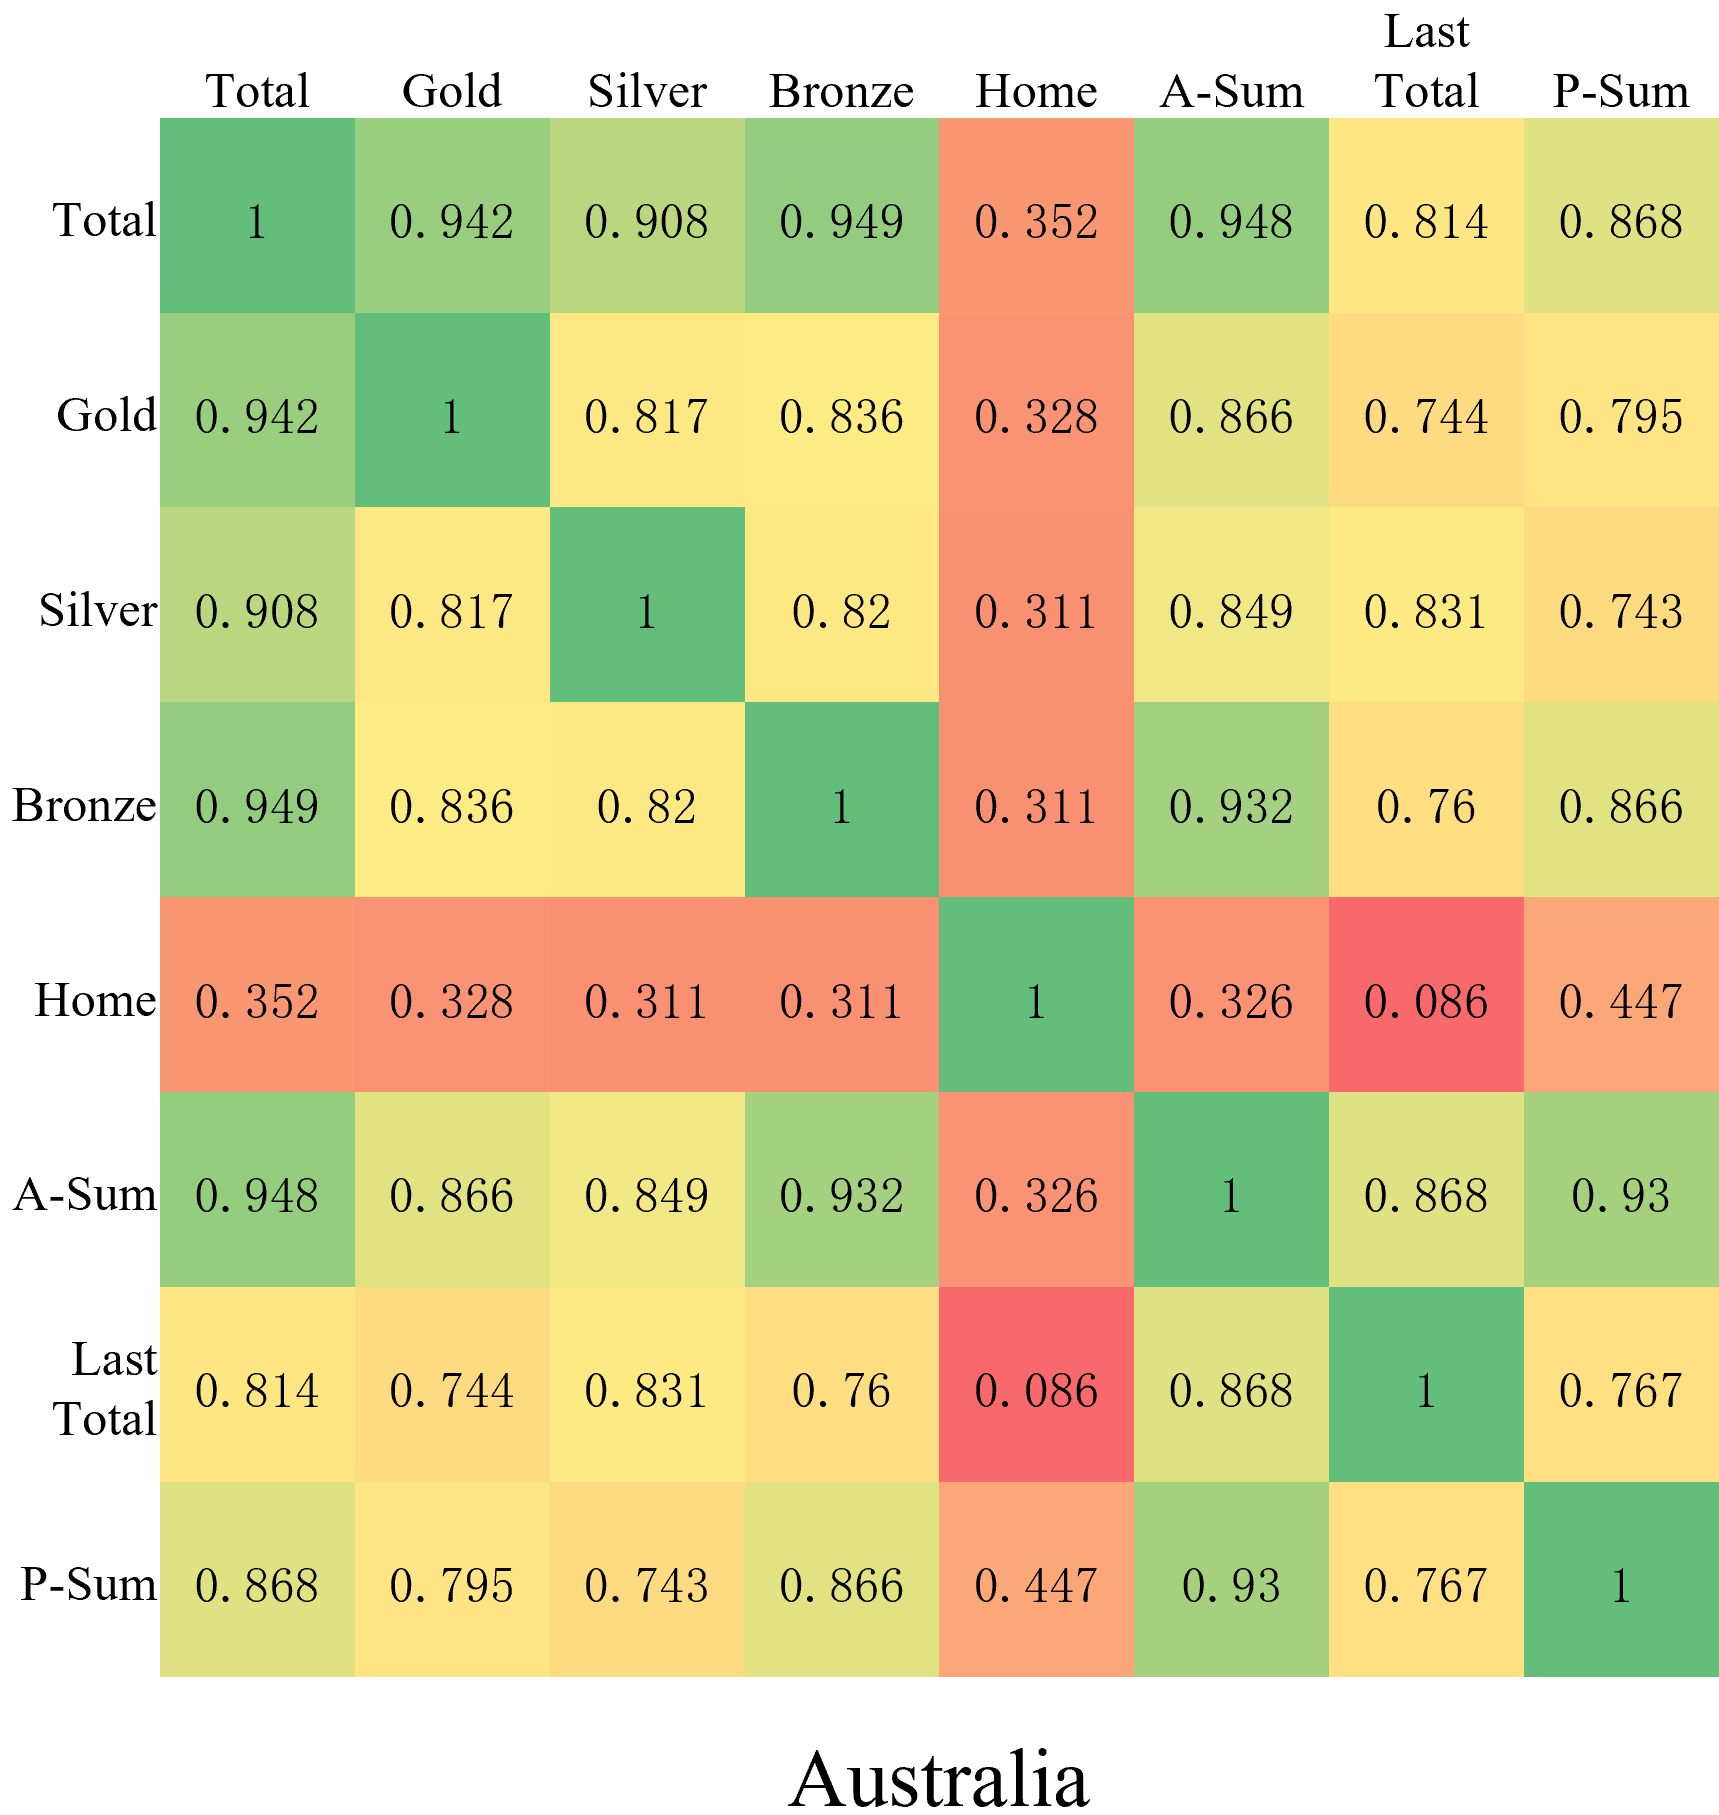
\includegraphics[width=1\linewidth]{Some_figures_4.png}
	\end{minipage}
	\caption{Correlation between the  number of Total Medal and other factors}
\end{figure}

%%普通表格
\begin{table}[h]  %h表示固定在当前位置
\centering        %设置居中
\caption{The calculating results}  %表标题
\vspace{0.15cm}
\label{tab2}                       %设置表的引用标签
\begin{tabular}{|c|c|c|}  %3个c表示3列, |可选, 表示绘制各列间的竖线
\hline                    %画横线
Variables & Values & Unit     \\ \hline  %各列间用&隔开
$A_1$     & 1.05   &   $m^2$  \\ \hline
$A_2$     & 2.24   &   $m^2$  \\ \hline
$\Phi_1$  & 189.00 &   $W$   \\ \hline
$\Phi_2$  & 43.47  &   $W$   \\ \hline
$\Phi$    & 232.47 &   $W$   \\ \hline
$q_m$     & 0.014  &   $g/s$ \\ \hline
\end{tabular}
\end{table}

\begin{equation}
P_{i, j}(t) = M_{i, j}(t) / S_{i, j}(t)
\end{equation}

$P_{i, j}(t)$

$M_{i, j}(t)$

$S_{i, j}(t)$

$\Delta P_{i, j} = P_{i, j}(t_{1}) - P_{i, j}(t_{0})$

\begin{equation}
\Delta P_{i, j} = \bar{P}_{i, j}^{after}(t_{0}) - \bar{P}_{i, j}^{before}(t_{0})
\end{equation}

\begin{equation}
\Delta M_{i, j}(t) = \Delta P_{i, j} \times A_{i, j}(t)
\end{equation}

$\Delta P_{i, j}$

\begin{equation}
MP^{i} = a_{1} ^ {i} + a_{2} ^{i}\times S_{1}\_Num^{i} + a_{3}^{i}\times P_{1}\_Num^{i} + a_{5}^{i}M
\end{equation}

$P_{1}\_Num^{i}=P_{ij} + \Delta P_{i, j} + P\_Num^{i}$

\begin{equation}
\Delta M=M_{c} - M_{b}
\end{equation}

\section{Task 2}

\begin{figure}[h] 
\centering
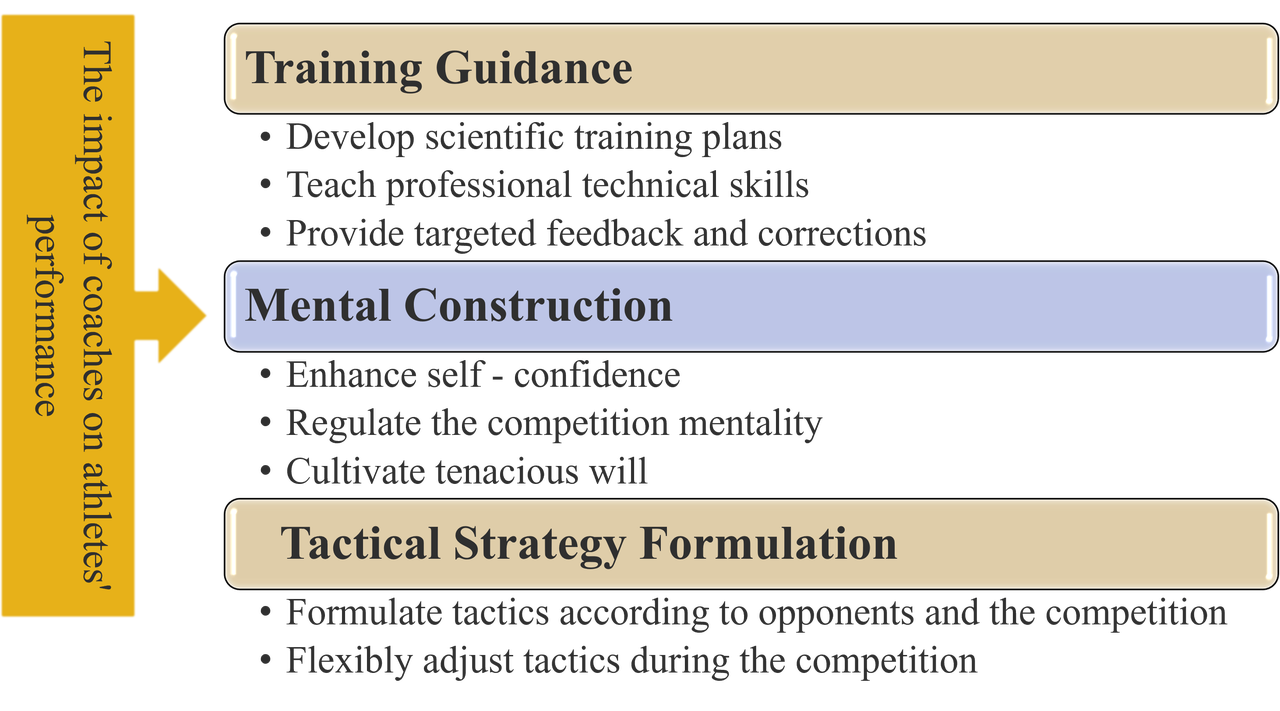
\includegraphics[width=8cm]{The impact of coaches on athletes' performance.png}
\caption{The impact of coaches on athletes' performance}
\end{figure}

\begin{figure}[h] 
\centering
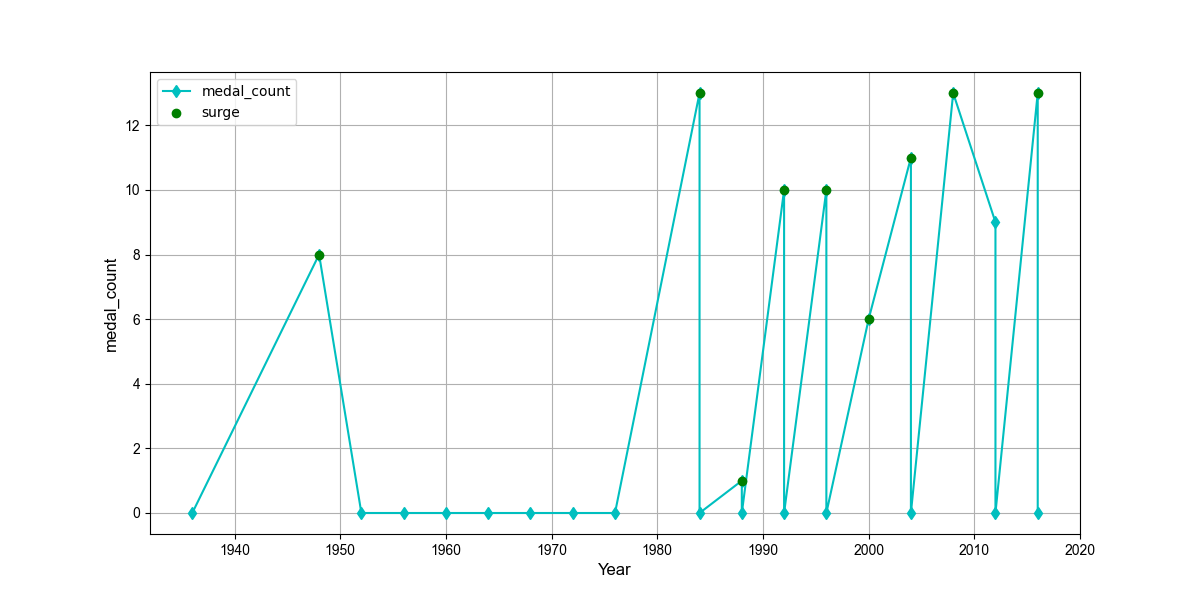
\includegraphics[width=8cm]{The number of Olympic medals won by the United States in women's gymnastics.png}
\caption{The number of Olympic medals won by the United States in women's gymnastics}
\end{figure}

\begin{figure}[h] 
\centering
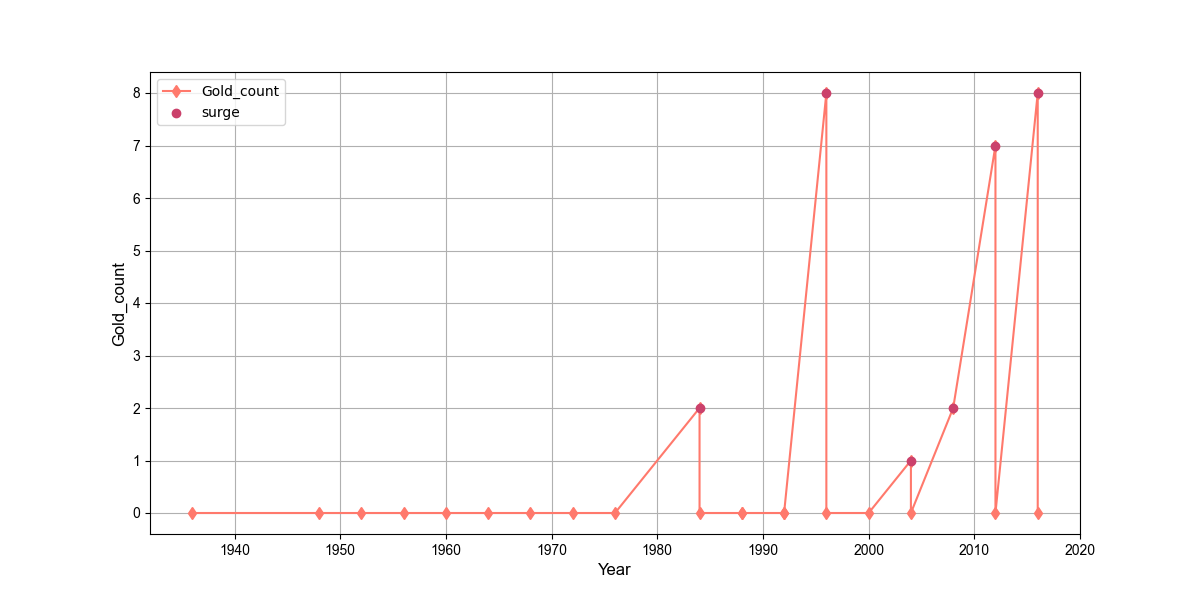
\includegraphics[width=8cm]{The number of Olympic gold medals won by the United States in women's gymnastics.png}
\caption{The number of Olympic gold medals won by the United States in women's gymnastics}
\end{figure}

\begin{figure}[h] 
\centering
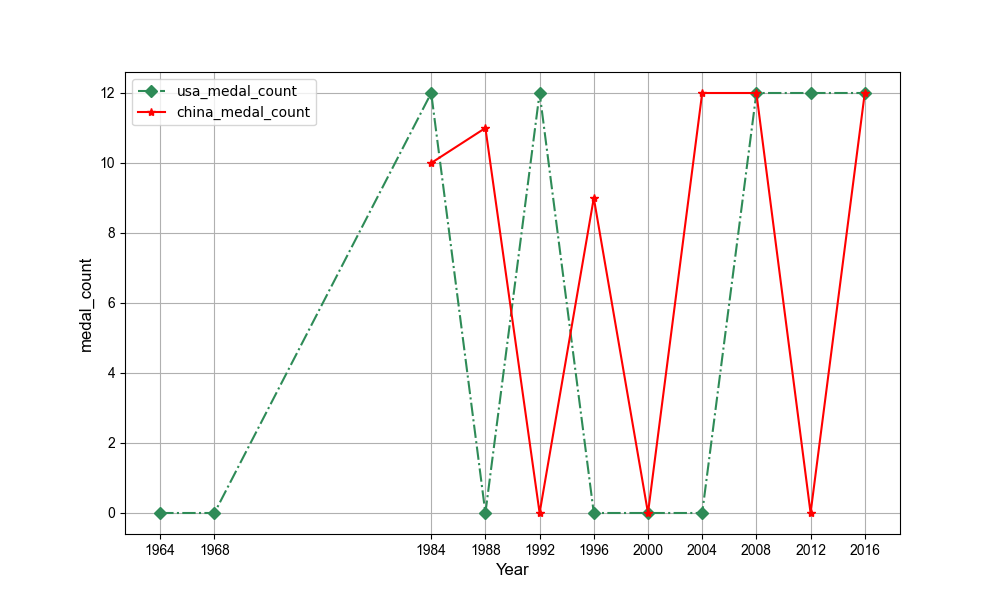
\includegraphics[width=8cm]{The number of Olympic medals won by China and the United States in women's volleyball.png}
\caption{The number of Olympic medals won by China and the United States in women's volleyball}
\end{figure}

\begin{table}
\centering
\caption{Table of variance analysis}
\begin{tabular}{|c|c|c|c|c|} 
\hline
\textcolor[rgb]{0.031,0.031,0.031}{~ Inspection value~~} & \textcolor[rgb]{0.031,0.031,0.031}{~ ~ Sample size~ ~~} & \textcolor[rgb]{0.031,0.031,0.031}{Standard deviation} & ~ z~~ & P        \\ 
\hline
1.12                                                     & 25                                                      & 2.538                                                  & 2.43  & 0.015**  \\ 
\hline
2.34                                                     & 25                                                      & 2.349                                                  & 3.26  & 0.011**  \\ 
\hline
2.12                                                     & 24                                                      & 1.956                                                  & 2.81  & 0.019**  \\
\hline
\end{tabular}
\end{table}

\begin{figure}[h] 
\centering
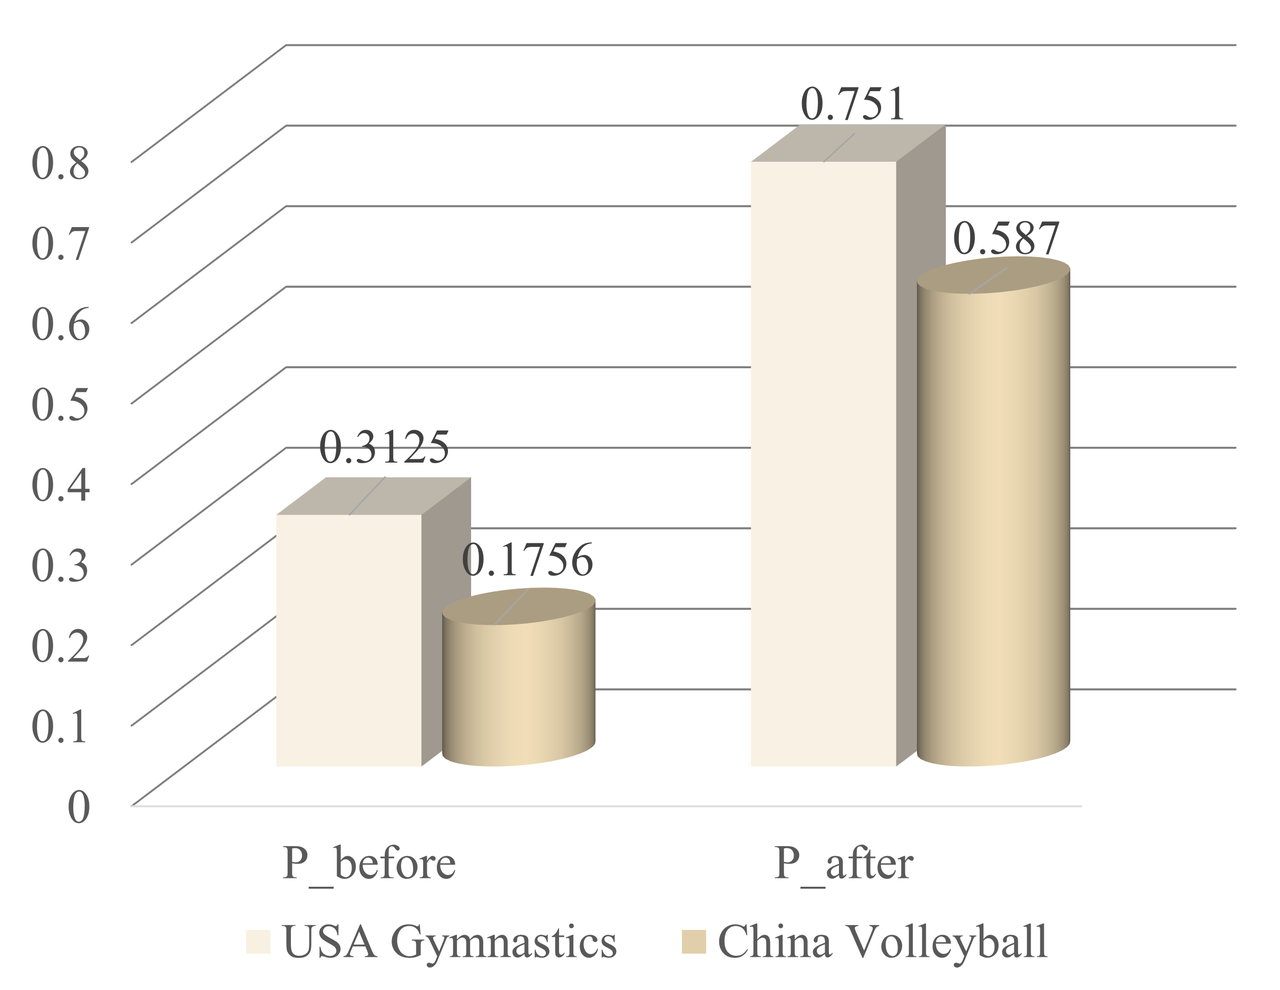
\includegraphics[width=8cm]{Changes in athlete performance levels in the two countries before and after coaching.png}
\caption{Description of the Differences}
\end{figure}

\begin{table}
\centering
\caption{Data files and encoding formats}
\begin{tabular}{|c|ccccc|} 
\hline
~ ~ Country~ ~~ & Pre\_Mc\_2028 & Rank & Pre\_Mb\_2028 & Rank & dete\_M  \\ 
\hline
Iran            & 5             & 46   & 8             & 32   & 3        \\
Ireland         & 4             & 54   & 7             & 33   & 3        \\
Uzbekistan      & 5             & 48   & 7             & 34   & 2        \\
\hline
\end{tabular}
\end{table}

$\Delta P_{i, j}$

\section{Task 3}

\subsection{Preliminary Analysis}
In the early years of the Olympics, the participation rate of women was extremely low. However, in recent years, with the advancement of civilization, women have gradually begun to emerge in the Olympic Games. The proportion of female participants in the total participation records has steadily increased, and by the 2024 Olympics, the participation rate of women is expected to be on par with that of men.

(figureXXX)

The majority of participants did not win any medals: 78.67\% of individuals (102,269 people) did not receive any medals. This observation reveals a clear Pareto effect, where 80\% of the medals are concentrated among 20\% of the participants, indicating that the vast majority of Olympic participants did not secure any medals.

A minority of individuals won medals: only 16.12\% of participants (20,957 people) earned one medal, while 3.50\% (4,546 people) won two medals. This demonstrates that the number of medal winners is relatively small, and the count decreases rapidly as the number of medals increases.

Sparsity of medal distribution: As the number of medals increases, the number of individuals who win medals decreases significantly. Only 0.14\% of participants (187 people) won five medals, and 0.09\% (113 people) won six medals, with the number of winners declining sharply after three medals.

A very small number of individuals achieved a high medal count: the data indicates that the number of participants who won ten or more medals is exceedingly rare, with only 17 individuals winning ten medals, and just one person winning 18 and 28 medals, respectively. This suggests that instances of winning a high number of medals are extremely uncommon within this dataset.

Distribution skewness: Overall, this distribution exhibits a pronounced positive skewness, indicating that the majority of individuals cluster around low medal counts (0-2 medals), while the distribution of higher medal counts is relatively sparse.

\begin{figure}[H] 
\centering
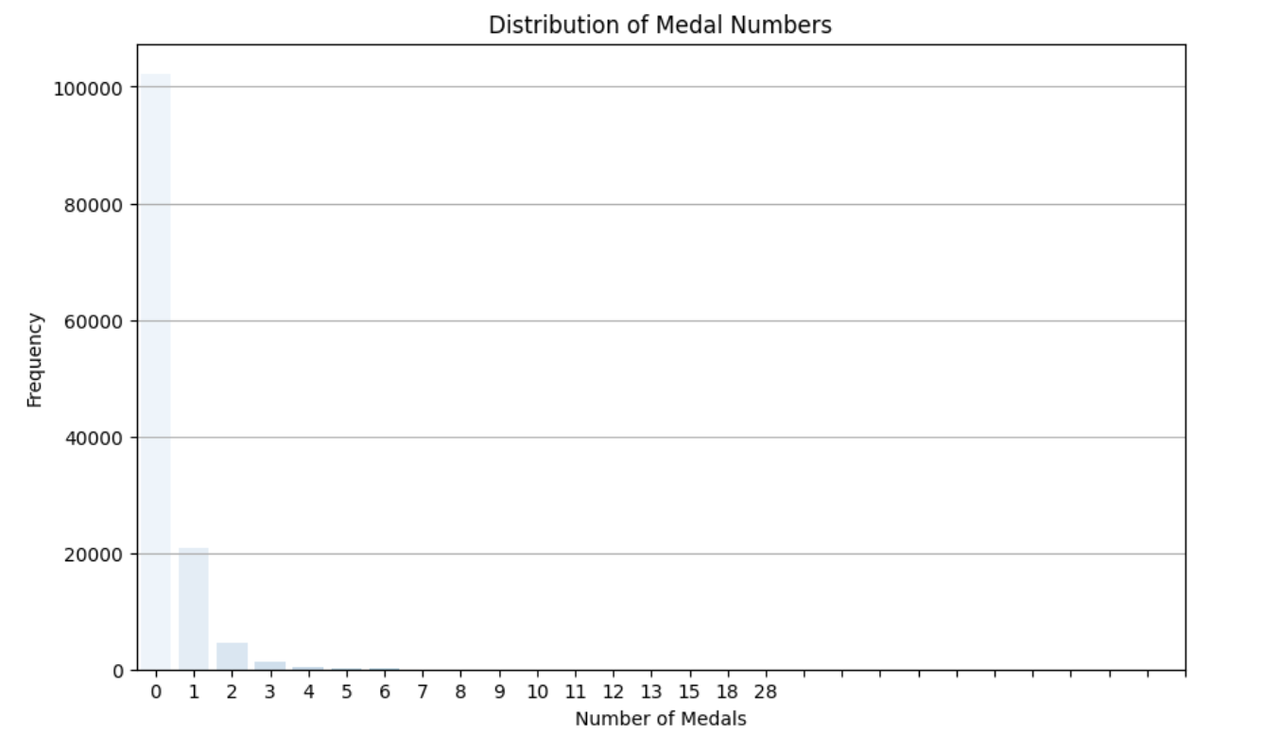
\includegraphics[width=12cm]{The changing participation rate of female athletes in various Olympic Games.png}
\caption{The changing participation rate of female athletes in various Olympic Games}
\end{figure}

We also observe that certain events are dominated by specific countries in terms of medal acquisition. For instance, countries such as the USA (Roque), SUI (Aeronautics), FRA (Croquet), GBR (Racquets), and ESP (Basque Pelota) have achieved a 100\% medal share in their respective sports events, indicating that these nations possess an absolute advantage in these particular competitions.

\begin{table}[H]
\centering
\caption{A descending list of the percentage of medals relative to the total number of medals}
\begin{tabular}{|c|c|c|c|c|} 
\hline
\textbf{~ NOC~~} & \textbf{Sport}        & \textbf{~ medal\_num~~} & \textbf{~ total\_medal\_num~~} & \textbf{~ percentage~~}  \\ 
\hline
USA              & Roque                 & 3                       & 3                              & 100                      \\ 
\hline
SUI              & Aeronautics           & 1                       & 1                              & 100                      \\ 
\hline
FRA              & Croquet               & 8                       & 8                              & 100                      \\ 
\hline
GBR              & Racquets              & 10                      & 10                             & 100                      \\ 
\hline
ESP              & Basque Pelota         & 2                       & 2                              & 100                      \\ 
\hline
GBR              & Cricket               & 21                      & 24                             & 87.5                     \\ 
\hline
GBR              & Motorboating          & 6                       & 7                              & 85.71429                 \\ 
\hline
USA              & Golf                  & 41                      & 58                             & 70.68966                 \\ 
\hline
GBR              & Jeu De Paume          & 2                       & 3                              & 66.66667                 \\ 
\hline
CAN              & Lacrosse              & 36                      & 60                             & 60                       \\ 
\hline
GER              & Alpinism              & 2                       & 4                              & 50                       \\ 
\hline
SUI              & Alpinism              & 2                       & 4                              & 50                       \\ 
\hline
GBR              & Polo                  & 30                      & 65                             & 46.15385                 \\ 
\hline
CHN              & Table Tennis          & 104                     & 228                            & 45.61404                 \\ 
\hline
CHN              & Trampoline Gym        & 5                       & 12                             & 41.66667                 \\ 
\hline
USA              & Ice Hockey            & 11                      & 27                             & 40.74074                 \\ 
\hline
CHN              & Badminton             & 83                      & 216                            & 38.42593                 \\ 
\hline
JPN              & Skateboarding         & 9                       & 24                             & 37.5                     \\ 
\hline
GBR              & Figure Skating        & 10                      & 27                             & 37.03704                 \\ 
\hline
CHN              & Trampolining          & 11                      & 30                             & 36.66667                 \\ 
\hline
SUI              & Cycling Mountain Bike & 4                       & 11                             & 36.36364                 \\
\hline
\end{tabular}
\end{table}
Additionally, there is a notable number of countries and events with moderate medal shares. For instance, CAN (Lacrosse) and GER, SUI (Alpinism) have medal shares ranging from 50\% to 60\%, demonstrating a certain level of competitiveness, although they do not reach a monopolistic status. Similarly, CHN (Table Tennis) and CHN (Badminton) account for 45.61\% and 38.43\% of the medals, respectively, indicating that China also performs strongly in these events.

Furthermore, some countries and events exhibit lower medal shares, such as USA (Ice Hockey) and JPN (Skateboarding), where the medal shares are below 40\%. This suggests that competition in these events is relatively intense, preventing any single nation from establishing a dominant position.

\begin{figure}[h] 
\centering
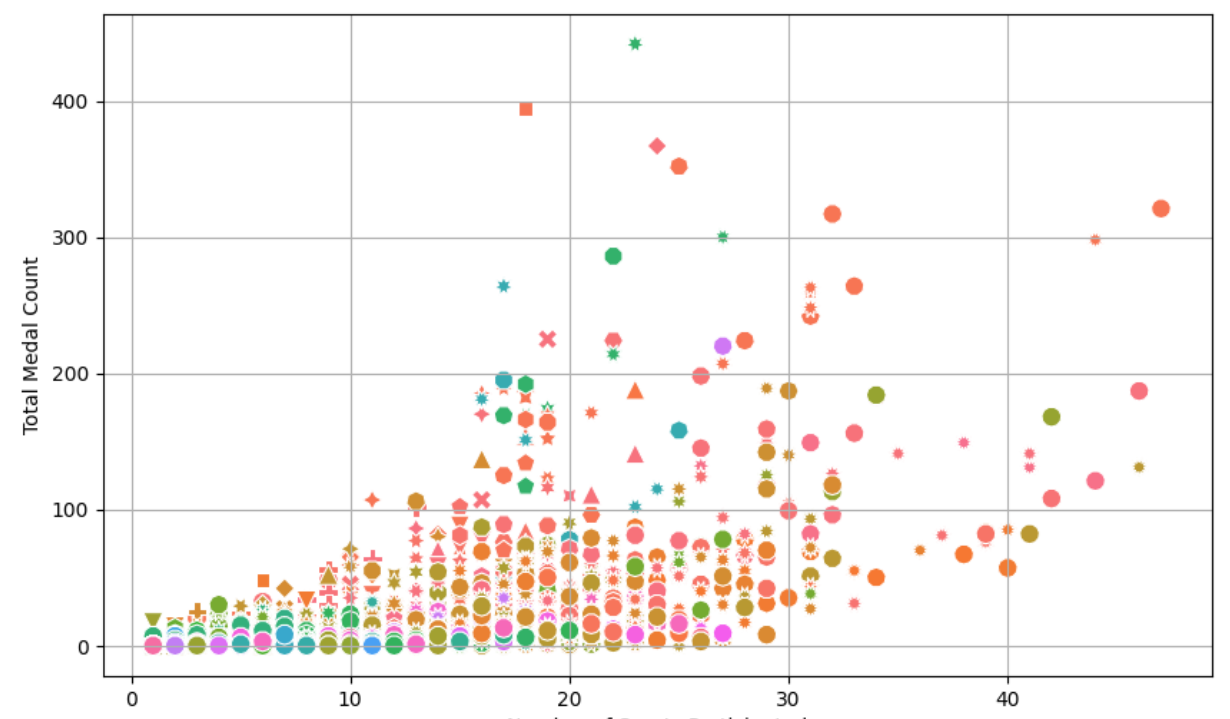
\includegraphics[width=12cm]{The relationship between the number of medals and the number of sports events participated in.png}
\caption{The relationship between the number of medals and the number of sports events participated in}
\end{figure}

From the above figure, it is evident that the diversification of sports events has a significant positive correlation with the number of Olympic medals obtained. To assess the relationship between the number of medals won by a country and the variety of sports events in which it participates, we employed correlation analysis. The results indicate that the Pearson correlation coefficient between the number of medals and the number of sports events participated in by the country is 0.6228, suggesting a strong positive correlation between the two variables.

\newpage

\subsection{Letter}

\begin{letter}{Enjoy Your Bath Time!}

From simulation results of real-life situations, we find it takes a period of time for the inflow hot water to spread throughout the bathtub. During this process, the bath water continues transferring heat into air, bathtub and the person in bathtub. The difference between heat transfer capacity makes the temperature of various areas to be different. So that it is difficult to get an evenly maintained temperature throughout the bath water.

In order to enjoy a comfortable bath with even temperature of bath water and without wasting too much water, we propose the following suggestions.

\begin{itemize}
\item Adding hot water consistently
\item Using smaller bathtub if possible
\item Decreasing motions during bath
\item Using bubble bath additives
\item Arranging more faucets of inflow
\end{itemize}

\vspace{\parskip}

Sincerely yours,

Team $\#$ 2517063

\end{letter}

\newpage

\section{Model Sensitivity Analysis}
$p(x)=\frac{1}{\sigma \sqrt{2\pi}}exp(-\frac{(x-\mu)^{2}}{2\sigma ^{2}})$

$\mu$

$\sigma$

$m_{x} = \frac{\left | Pre_{\_New} - Pre_{\_Old}\right |}{Pre_{\_Old}}\times 100\%$

\section{Model Evaluation}
\subsection{Strengths}
\begin{itemize}
\item XXXXX

\item XXXX

\item XXXXX
\end{itemize}

\begin{table}
\centering
\caption{Description of the Advantages and Disadvantages of Events}
\begin{tabular}{|c|c|c|} 
\hline
\textbf{~ NOC~~}     & \textbf{~ ~ A\_Sport~ ~~} & \textbf{~ ~ ~B\_Sport~ ~~}  \\ 
\hline
\multirow{2}{*}{IRL} & Aquatics                  & Boxing                      \\ 
\cline{2-3}
                     & Athletics                 & Rowing                      \\ 
\hline
\multirow{2}{*}{UZB} & Boxing                    & Gymnastics                  \\ 
\cline{2-3}
                     & Taekwondo                 & Judo                        \\ 
\hline
\multirow{3}{*}{IRI} & Karate                    & Athletics                   \\ 
\cline{2-3}
                     & Shooting                  & Weightlifting               \\ 
\cline{2-3}
                     & Taekwondo                 & Wrestling                   \\
\hline
\end{tabular}
\end{table}

\subsection{Weaknesses}

\begin{itemize}
\item XXXXX

\item XXXX

\item XXXXX
\end{itemize}

\newpage

\begin{thebibliography}{99}
\addcontentsline{toc}{section}{Reference}

\bibitem{1} Gao Xuan. Analysis of Competitive Performance in Women's Throwing Events in the Last Five Olympic Games and Prediction for the Tokyo Olympic Games [D]. Beijing Sport University, 2018.(In Chinese) 
\bibitem{2} Li Ran. Research on the Competitive Performance of Women's Throwing Events from the 24th to the 32nd Olympic Games and Prediction of the Results for the Paris Olympic Games [D]. Qufu Normal University, 2023. DOI: 10.27267/d.cnki.gqfsu.2023.000828.(In Chinese) 
\bibitem{3} May T P ,Keenan D T ,Potts R , et al.The Sydney 2000 Olympic Games Forecast Demonstration Project: Forecasting, observing network infrastructure, and data processing issues[J].American Meteorological Society,2004,19(1):115-130.
\bibitem{4} Wang Guofan, Zhao Wu, Liu Xujun, et al. Research on Olympic Game Results Prediction Based on GA and Regression Analysis [J]. China Sports Science and Technology, 2011, 47(01): 4-8 + 16. DOI: 10.16470/j.csst.2011.01.002.(In Chinese) 
\bibitem{5} Yang Qinwei. Multivariate Linear Regression Model Predicting the Results of the 2020 Olympic Games [J]. Electronic Production, 2018, (Z2): 121-123. DOI: 10.16589/j.cnki.cn11-3571/tn.2018.z2.058.(In Chinese)
\bibitem{6} Zhang Haibo, Zhao Huancheng. Prediction of the Number of Gold Medals for the Chinese Team in the Beijing Olympic Games [J]. Statistics and Decision, 2008, (15): 76-77. (In Chinese)

\end{thebibliography}

\begin{appendices}

\section{First appendix}

In addition, your report must include a letter to the Chief Financial Officer (CFO) of the Goodgrant Foundation, Mr. Alpha Chiang, that describes the optimal investment strategy, your modeling approach and major results, and a brief discussion of your proposed concept of a return-on-investment (ROI). This letter should be no more than two pages in length.

Here are simulation programmes we used in our model as follow.\\

\textbf{\textcolor[rgb]{0.98,0.00,0.00}{Input matlab source:}}
\lstinputlisting[language=Matlab]{./code/mcmthesis-matlab1.m}

\section{Second appendix}

some more text \textcolor[rgb]{0.98,0.00,0.00}{\textbf{Input C++ source:}}
\lstinputlisting[language=C++]{./code/mcmthesis-sudoku.cpp}

\end{appendices}
\end{document}
%%
%% This work consists of these files mcmthesis.dtx,
%%                                   figures/ and
%%                                   code/,
%% and the derived files             mcmthesis.cls,
%%                                   mcmthesis-demo.tex,
%%                                   README,
%%                                   LICENSE,
%%                                   mcmthesis.pdf and
%%                                   mcmthesis-demo.pdf.
%%
%% End of file `mcmthesis-demo.tex'.
